\documentclass[twoside]{book}

% Packages required by doxygen
\usepackage{calc}
\usepackage{doxygen}
\usepackage{graphicx}
\usepackage[utf8]{inputenc}
\usepackage{makeidx}
\usepackage{multicol}
\usepackage{multirow}
\usepackage{textcomp}
\usepackage[table]{xcolor}

% Font selection
\usepackage[T1]{fontenc}
\usepackage{mathptmx}
\usepackage[scaled=.90]{helvet}
\usepackage{courier}
\usepackage{amssymb}
\usepackage{sectsty}
\renewcommand{\familydefault}{\sfdefault}
\allsectionsfont{%
  \fontseries{bc}\selectfont%
  \color{darkgray}%
}
\renewcommand{\DoxyLabelFont}{%
  \fontseries{bc}\selectfont%
  \color{darkgray}%
}

% Page & text layout
\usepackage{geometry}
\geometry{%
  a4paper,%
  top=2.5cm,%
  bottom=2.5cm,%
  left=2.5cm,%
  right=2.5cm%
}
\tolerance=750
\hfuzz=15pt
\hbadness=750
\setlength{\emergencystretch}{15pt}
\setlength{\parindent}{0cm}
\setlength{\parskip}{0.2cm}
\makeatletter
\renewcommand{\paragraph}{%
  \@startsection{paragraph}{4}{0ex}{-1.0ex}{1.0ex}{%
    \normalfont\normalsize\bfseries\SS@parafont%
  }%
}
\renewcommand{\subparagraph}{%
  \@startsection{subparagraph}{5}{0ex}{-1.0ex}{1.0ex}{%
    \normalfont\normalsize\bfseries\SS@subparafont%
  }%
}
\makeatother

% Headers & footers
\usepackage{fancyhdr}
\pagestyle{fancyplain}
\fancyhead[LE]{\fancyplain{}{\bfseries\thepage}}
\fancyhead[CE]{\fancyplain{}{}}
\fancyhead[RE]{\fancyplain{}{\bfseries\leftmark}}
\fancyhead[LO]{\fancyplain{}{\bfseries\rightmark}}
\fancyhead[CO]{\fancyplain{}{}}
\fancyhead[RO]{\fancyplain{}{\bfseries\thepage}}
\fancyfoot[LE]{\fancyplain{}{}}
\fancyfoot[CE]{\fancyplain{}{}}
\fancyfoot[RE]{\fancyplain{}{\bfseries\scriptsize Generated on Sun Jun 29 2014 14:07:52 for mupdf-qt by Doxygen }}
\fancyfoot[LO]{\fancyplain{}{\bfseries\scriptsize Generated on Sun Jun 29 2014 14:07:52 for mupdf-qt by Doxygen }}
\fancyfoot[CO]{\fancyplain{}{}}
\fancyfoot[RO]{\fancyplain{}{}}
\renewcommand{\footrulewidth}{0.4pt}
\renewcommand{\chaptermark}[1]{%
  \markboth{#1}{}%
}
\renewcommand{\sectionmark}[1]{%
  \markright{\thesection\ #1}%
}

% Indices & bibliography
\usepackage{natbib}
\usepackage[titles]{tocloft}
\setcounter{tocdepth}{3}
\setcounter{secnumdepth}{5}
\makeindex

% Hyperlinks (required, but should be loaded last)
\usepackage{ifpdf}
\ifpdf
  \usepackage[pdftex,pagebackref=true]{hyperref}
\else
  \usepackage[ps2pdf,pagebackref=true]{hyperref}
\fi
\hypersetup{%
  colorlinks=true,%
  linkcolor=blue,%
  citecolor=blue,%
  unicode%
}

% Custom commands
\newcommand{\clearemptydoublepage}{%
  \newpage{\pagestyle{empty}\cleardoublepage}%
}


%===== C O N T E N T S =====

\begin{document}

% Titlepage & ToC
\hypersetup{pageanchor=false}
\pagenumbering{roman}
\begin{titlepage}
\vspace*{7cm}
\begin{center}%
{\Large mupdf-\/qt }\\
\vspace*{1cm}
{\large Generated by Doxygen 1.8.4}\\
\vspace*{0.5cm}
{\small Sun Jun 29 2014 14:07:52}\\
\end{center}
\end{titlepage}
\clearemptydoublepage
\tableofcontents
\clearemptydoublepage
\pagenumbering{arabic}
\hypersetup{pageanchor=true}

%--- Begin generated contents ---
\chapter{Namespace Index}
\section{Namespace List}
Here is a list of all namespaces with brief descriptions\-:\begin{DoxyCompactList}
\item\contentsline{section}{\hyperlink{namespace_mu_p_d_f}{Mu\-P\-D\-F} }{\pageref{namespace_mu_p_d_f}}{}
\end{DoxyCompactList}

\chapter{Hierarchical Index}
\section{Class Hierarchy}
This inheritance list is sorted roughly, but not completely, alphabetically\-:\begin{DoxyCompactList}
\item \contentsline{section}{Mu\-P\-D\-F\-:\-:Document}{\pageref{class_mu_p_d_f_1_1_document}}{}
\item \contentsline{section}{Mu\-P\-D\-F\-:\-:Link}{\pageref{class_mu_p_d_f_1_1_link}}{}
\begin{DoxyCompactList}
\item \contentsline{section}{Mu\-P\-D\-F\-:\-:Link\-Goto}{\pageref{class_mu_p_d_f_1_1_link_goto}}{}
\begin{DoxyCompactList}
\item \contentsline{section}{Mu\-P\-D\-F\-:\-:Link\-Goto\-R}{\pageref{class_mu_p_d_f_1_1_link_goto_r}}{}
\end{DoxyCompactList}
\item \contentsline{section}{Mu\-P\-D\-F\-:\-:Link\-Launch}{\pageref{class_mu_p_d_f_1_1_link_launch}}{}
\item \contentsline{section}{Mu\-P\-D\-F\-:\-:Link\-Named}{\pageref{class_mu_p_d_f_1_1_link_named}}{}
\item \contentsline{section}{Mu\-P\-D\-F\-:\-:Link\-U\-R\-I}{\pageref{class_mu_p_d_f_1_1_link_u_r_i}}{}
\end{DoxyCompactList}
\item \contentsline{section}{Mu\-P\-D\-F\-:\-:Outline}{\pageref{class_mu_p_d_f_1_1_outline}}{}
\item \contentsline{section}{Mu\-P\-D\-F\-:\-:Outline\-Item}{\pageref{class_mu_p_d_f_1_1_outline_item}}{}
\item \contentsline{section}{Mu\-P\-D\-F\-:\-:Page}{\pageref{class_mu_p_d_f_1_1_page}}{}
\item \contentsline{section}{Mu\-P\-D\-F\-:\-:Text\-Box}{\pageref{class_mu_p_d_f_1_1_text_box}}{}
\end{DoxyCompactList}

\chapter{Class Index}
\section{Class List}
Here are the classes, structs, unions and interfaces with brief descriptions\-:\begin{DoxyCompactList}
\item\contentsline{section}{\hyperlink{class_mu_p_d_f_1_1_document}{Mu\-P\-D\-F\-::\-Document} }{\pageref{class_mu_p_d_f_1_1_document}}{}
\item\contentsline{section}{\hyperlink{class_mu_p_d_f_1_1_link}{Mu\-P\-D\-F\-::\-Link} }{\pageref{class_mu_p_d_f_1_1_link}}{}
\item\contentsline{section}{\hyperlink{class_mu_p_d_f_1_1_link_goto}{Mu\-P\-D\-F\-::\-Link\-Goto} \\*Goto a position in current file }{\pageref{class_mu_p_d_f_1_1_link_goto}}{}
\item\contentsline{section}{\hyperlink{class_mu_p_d_f_1_1_link_goto_r}{Mu\-P\-D\-F\-::\-Link\-Goto\-R} \\*Goto a position in another file }{\pageref{class_mu_p_d_f_1_1_link_goto_r}}{}
\item\contentsline{section}{\hyperlink{class_mu_p_d_f_1_1_link_launch}{Mu\-P\-D\-F\-::\-Link\-Launch} \\*Launch a file (a document or a executable) }{\pageref{class_mu_p_d_f_1_1_link_launch}}{}
\item\contentsline{section}{\hyperlink{class_mu_p_d_f_1_1_link_named}{Mu\-P\-D\-F\-::\-Link\-Named} \\*Named action to perform }{\pageref{class_mu_p_d_f_1_1_link_named}}{}
\item\contentsline{section}{\hyperlink{class_mu_p_d_f_1_1_link_u_r_i}{Mu\-P\-D\-F\-::\-Link\-U\-R\-I} \\*A U\-R\-I link }{\pageref{class_mu_p_d_f_1_1_link_u_r_i}}{}
\item\contentsline{section}{\hyperlink{class_mu_p_d_f_1_1_outline}{Mu\-P\-D\-F\-::\-Outline} \\*A tree of the outline of a document (also known as table of contents) }{\pageref{class_mu_p_d_f_1_1_outline}}{}
\item\contentsline{section}{\hyperlink{class_mu_p_d_f_1_1_outline_item}{Mu\-P\-D\-F\-::\-Outline\-Item} \\*A outline item }{\pageref{class_mu_p_d_f_1_1_outline_item}}{}
\item\contentsline{section}{\hyperlink{class_mu_p_d_f_1_1_page}{Mu\-P\-D\-F\-::\-Page} }{\pageref{class_mu_p_d_f_1_1_page}}{}
\end{DoxyCompactList}

\chapter{File Index}
\section{File List}
Here is a list of all files with brief descriptions\-:\begin{DoxyCompactList}
\item\contentsline{section}{libmupdf-\/qt/\hyperlink{mupdf-document_8cpp}{mupdf-\/document.\-cpp} }{\pageref{mupdf-document_8cpp}}{}
\item\contentsline{section}{libmupdf-\/qt/\hyperlink{mupdf-document_8h}{mupdf-\/document.\-h} }{\pageref{mupdf-document_8h}}{}
\item\contentsline{section}{libmupdf-\/qt/\hyperlink{mupdf-link_8cpp}{mupdf-\/link.\-cpp} }{\pageref{mupdf-link_8cpp}}{}
\item\contentsline{section}{libmupdf-\/qt/\hyperlink{mupdf-link_8h}{mupdf-\/link.\-h} }{\pageref{mupdf-link_8h}}{}
\item\contentsline{section}{libmupdf-\/qt/\hyperlink{mupdf-outline_8cpp}{mupdf-\/outline.\-cpp} }{\pageref{mupdf-outline_8cpp}}{}
\item\contentsline{section}{libmupdf-\/qt/\hyperlink{mupdf-outline_8h}{mupdf-\/outline.\-h} }{\pageref{mupdf-outline_8h}}{}
\item\contentsline{section}{libmupdf-\/qt/\hyperlink{mupdf-page_8cpp}{mupdf-\/page.\-cpp} }{\pageref{mupdf-page_8cpp}}{}
\item\contentsline{section}{libmupdf-\/qt/\hyperlink{mupdf-page_8h}{mupdf-\/page.\-h} }{\pageref{mupdf-page_8h}}{}
\item\contentsline{section}{libmupdf-\/qt/\hyperlink{mupdf-qt_8h}{mupdf-\/qt.\-h} }{\pageref{mupdf-qt_8h}}{}
\end{DoxyCompactList}

\chapter{Namespace Documentation}
\hypertarget{namespace_mu_p_d_f}{\section{Mu\-P\-D\-F Namespace Reference}
\label{namespace_mu_p_d_f}\index{Mu\-P\-D\-F@{Mu\-P\-D\-F}}
}
\subsection*{Classes}
\begin{DoxyCompactItemize}
\item 
class \hyperlink{class_mu_p_d_f_1_1_document}{Document}
\item 
class \hyperlink{class_mu_p_d_f_1_1_link}{Link}
\item 
class \hyperlink{class_mu_p_d_f_1_1_link_goto}{Link\-Goto}
\begin{DoxyCompactList}\small\item\em Goto a position in current file. \end{DoxyCompactList}\item 
class \hyperlink{class_mu_p_d_f_1_1_link_u_r_i}{Link\-U\-R\-I}
\begin{DoxyCompactList}\small\item\em A U\-R\-I link. \end{DoxyCompactList}\item 
class \hyperlink{class_mu_p_d_f_1_1_link_launch}{Link\-Launch}
\begin{DoxyCompactList}\small\item\em Launch a file (a document or a executable). \end{DoxyCompactList}\item 
class \hyperlink{class_mu_p_d_f_1_1_link_named}{Link\-Named}
\begin{DoxyCompactList}\small\item\em Named action to perform. \end{DoxyCompactList}\item 
class \hyperlink{class_mu_p_d_f_1_1_link_goto_r}{Link\-Goto\-R}
\begin{DoxyCompactList}\small\item\em Goto a position in another file. \end{DoxyCompactList}\item 
class \hyperlink{class_mu_p_d_f_1_1_outline}{Outline}
\begin{DoxyCompactList}\small\item\em A tree of the outline of a document (also known as table of contents). \end{DoxyCompactList}\item 
class \hyperlink{class_mu_p_d_f_1_1_outline_item}{Outline\-Item}
\begin{DoxyCompactList}\small\item\em A outline item. \end{DoxyCompactList}\item 
class \hyperlink{class_mu_p_d_f_1_1_page}{Page}
\begin{DoxyCompactList}\small\item\em A page. \end{DoxyCompactList}\item 
class \hyperlink{class_mu_p_d_f_1_1_text_box}{Text\-Box}
\begin{DoxyCompactList}\small\item\em A text box. \end{DoxyCompactList}\end{DoxyCompactItemize}
\subsection*{Functions}
\begin{DoxyCompactItemize}
\item 
\hyperlink{class_mu_p_d_f_1_1_document}{Document} $\ast$ \hyperlink{namespace_mu_p_d_f_a5cf746094bc9648aca0d4a83e3ac44b3}{load\-Document} (const Q\-String \&file\-Path)
\begin{DoxyCompactList}\small\item\em Load a document. \end{DoxyCompactList}\item 
\hyperlink{class_mu_p_d_f_1_1_document}{Document} $\ast$ \hyperlink{namespace_mu_p_d_f_a294a09188a3dcab290679752dfc8d52b}{load\-Document} (const Q\-Byte\-Array \&bytes)
\begin{DoxyCompactList}\small\item\em Load a document. \end{DoxyCompactList}\item 
Q\-Point\-F \hyperlink{namespace_mu_p_d_f_a40833e5e56d0d7d44cba455e4186d5e4}{map\-To\-Origin} (const Q\-Point\-F \&pos, float scale\-X, float scale\-Y, float rotation=0.\-0f)
\begin{DoxyCompactList}\small\item\em Map from a transformed point to the original point. \end{DoxyCompactList}\item 
Q\-Size\-F \hyperlink{namespace_mu_p_d_f_ae91a73bb4e3e4c10eb54c07ab9be9cf7}{map\-To\-Origin} (const Q\-Size\-F \&size, float scale\-X, float scale\-Y, float rotation=0.\-0f)
\begin{DoxyCompactList}\small\item\em Map from a transformed size to the original size. \end{DoxyCompactList}\item 
Q\-Rect\-F \hyperlink{namespace_mu_p_d_f_a2132cae17dab8f9896ec0c83f0c2173c}{map\-To\-Origin} (const Q\-Rect\-F \&rect, float scale\-X, float scale\-Y, float rotation=0.\-0f)
\begin{DoxyCompactList}\small\item\em Map from a transformed rect to the original rect. \end{DoxyCompactList}\item 
Q\-Point\-F \hyperlink{namespace_mu_p_d_f_ad849bcc678dd57c1f12619f9554e6aba}{map\-From\-Origin} (const Q\-Point\-F \&pos, float scale\-X, float scale\-Y, float rotation=0.\-0f)
\begin{DoxyCompactList}\small\item\em Map from a original point to the transformed point. \end{DoxyCompactList}\item 
Q\-Size\-F \hyperlink{namespace_mu_p_d_f_a6c6cac36e5a30ed75952a619b19d33aa}{map\-From\-Origin} (const Q\-Size\-F \&size, float scale\-X, float scale\-Y, float rotation=0.\-0f)
\begin{DoxyCompactList}\small\item\em Map from a original size to the transformed size. \end{DoxyCompactList}\item 
Q\-Rect\-F \hyperlink{namespace_mu_p_d_f_a2f2a28dce44170175d3e9ba9601478ea}{map\-From\-Origin} (const Q\-Rect\-F \&rect, float scale\-X, float scale\-Y, float rotation=0.\-0f)
\begin{DoxyCompactList}\small\item\em Map from a original rect to the transformed rect. \end{DoxyCompactList}\end{DoxyCompactItemize}


\subsection{Function Documentation}
\hypertarget{namespace_mu_p_d_f_a5cf746094bc9648aca0d4a83e3ac44b3}{\index{Mu\-P\-D\-F@{Mu\-P\-D\-F}!load\-Document@{load\-Document}}
\index{load\-Document@{load\-Document}!MuPDF@{Mu\-P\-D\-F}}
\subsubsection[{load\-Document}]{\setlength{\rightskip}{0pt plus 5cm}{\bf Document} $\ast$ Mu\-P\-D\-F\-::load\-Document (
\begin{DoxyParamCaption}
\item[{const Q\-String \&}]{file\-Path}
\end{DoxyParamCaption}
)}}\label{namespace_mu_p_d_f_a5cf746094bc9648aca0d4a83e3ac44b3}


Load a document. 


\begin{DoxyParams}{Parameters}
{\em file\-Path} & document path\\
\hline
\end{DoxyParams}
\begin{DoxyReturn}{Returns}
N\-U\-L\-L if failed (Note\-: you need delete manually when it's useless) 
\end{DoxyReturn}


Definition at line 23 of file mupdf-\/document.\-cpp.

\hypertarget{namespace_mu_p_d_f_a294a09188a3dcab290679752dfc8d52b}{\index{Mu\-P\-D\-F@{Mu\-P\-D\-F}!load\-Document@{load\-Document}}
\index{load\-Document@{load\-Document}!MuPDF@{Mu\-P\-D\-F}}
\subsubsection[{load\-Document}]{\setlength{\rightskip}{0pt plus 5cm}{\bf Document} $\ast$ Mu\-P\-D\-F\-::load\-Document (
\begin{DoxyParamCaption}
\item[{const Q\-Byte\-Array \&}]{bytes}
\end{DoxyParamCaption}
)}}\label{namespace_mu_p_d_f_a294a09188a3dcab290679752dfc8d52b}


Load a document. 


\begin{DoxyParams}{Parameters}
{\em bytes} & document data\\
\hline
\end{DoxyParams}
\begin{DoxyReturn}{Returns}
N\-U\-L\-L if failed (Note\-: you need delete manually when it's useless) 
\end{DoxyReturn}


Definition at line 49 of file mupdf-\/document.\-cpp.

\hypertarget{namespace_mu_p_d_f_ad849bcc678dd57c1f12619f9554e6aba}{\index{Mu\-P\-D\-F@{Mu\-P\-D\-F}!map\-From\-Origin@{map\-From\-Origin}}
\index{map\-From\-Origin@{map\-From\-Origin}!MuPDF@{Mu\-P\-D\-F}}
\subsubsection[{map\-From\-Origin}]{\setlength{\rightskip}{0pt plus 5cm}Q\-Point\-F Mu\-P\-D\-F\-::map\-From\-Origin (
\begin{DoxyParamCaption}
\item[{const Q\-Point\-F \&}]{pos, }
\item[{float}]{scale\-X, }
\item[{float}]{scale\-Y, }
\item[{float}]{rotation = {\ttfamily 0.0f}}
\end{DoxyParamCaption}
)}}\label{namespace_mu_p_d_f_ad849bcc678dd57c1f12619f9554e6aba}


Map from a original point to the transformed point. 

\begin{DoxyReturn}{Returns}
The transformed point. 
\end{DoxyReturn}


Definition at line 121 of file mupdf-\/page.\-cpp.

\hypertarget{namespace_mu_p_d_f_a6c6cac36e5a30ed75952a619b19d33aa}{\index{Mu\-P\-D\-F@{Mu\-P\-D\-F}!map\-From\-Origin@{map\-From\-Origin}}
\index{map\-From\-Origin@{map\-From\-Origin}!MuPDF@{Mu\-P\-D\-F}}
\subsubsection[{map\-From\-Origin}]{\setlength{\rightskip}{0pt plus 5cm}Q\-Size\-F Mu\-P\-D\-F\-::map\-From\-Origin (
\begin{DoxyParamCaption}
\item[{const Q\-Size\-F \&}]{size, }
\item[{float}]{scale\-X, }
\item[{float}]{scale\-Y, }
\item[{float}]{rotation = {\ttfamily 0.0f}}
\end{DoxyParamCaption}
)}}\label{namespace_mu_p_d_f_a6c6cac36e5a30ed75952a619b19d33aa}


Map from a original size to the transformed size. 

\begin{DoxyReturn}{Returns}
The transformed size. 
\end{DoxyReturn}


Definition at line 138 of file mupdf-\/page.\-cpp.

\hypertarget{namespace_mu_p_d_f_a2f2a28dce44170175d3e9ba9601478ea}{\index{Mu\-P\-D\-F@{Mu\-P\-D\-F}!map\-From\-Origin@{map\-From\-Origin}}
\index{map\-From\-Origin@{map\-From\-Origin}!MuPDF@{Mu\-P\-D\-F}}
\subsubsection[{map\-From\-Origin}]{\setlength{\rightskip}{0pt plus 5cm}Q\-Rect\-F Mu\-P\-D\-F\-::map\-From\-Origin (
\begin{DoxyParamCaption}
\item[{const Q\-Rect\-F \&}]{rect, }
\item[{float}]{scale\-X, }
\item[{float}]{scale\-Y, }
\item[{float}]{rotation = {\ttfamily 0.0f}}
\end{DoxyParamCaption}
)}}\label{namespace_mu_p_d_f_a2f2a28dce44170175d3e9ba9601478ea}


Map from a original rect to the transformed rect. 

\begin{DoxyReturn}{Returns}
The transformed rect. 
\end{DoxyReturn}


Definition at line 155 of file mupdf-\/page.\-cpp.

\hypertarget{namespace_mu_p_d_f_a40833e5e56d0d7d44cba455e4186d5e4}{\index{Mu\-P\-D\-F@{Mu\-P\-D\-F}!map\-To\-Origin@{map\-To\-Origin}}
\index{map\-To\-Origin@{map\-To\-Origin}!MuPDF@{Mu\-P\-D\-F}}
\subsubsection[{map\-To\-Origin}]{\setlength{\rightskip}{0pt plus 5cm}Q\-Point\-F Mu\-P\-D\-F\-::map\-To\-Origin (
\begin{DoxyParamCaption}
\item[{const Q\-Point\-F \&}]{pos, }
\item[{float}]{scale\-X, }
\item[{float}]{scale\-Y, }
\item[{float}]{rotation = {\ttfamily 0.0f}}
\end{DoxyParamCaption}
)}}\label{namespace_mu_p_d_f_a40833e5e56d0d7d44cba455e4186d5e4}


Map from a transformed point to the original point. 

\begin{DoxyReturn}{Returns}
The original point. 
\end{DoxyReturn}


Definition at line 56 of file mupdf-\/page.\-cpp.

\hypertarget{namespace_mu_p_d_f_ae91a73bb4e3e4c10eb54c07ab9be9cf7}{\index{Mu\-P\-D\-F@{Mu\-P\-D\-F}!map\-To\-Origin@{map\-To\-Origin}}
\index{map\-To\-Origin@{map\-To\-Origin}!MuPDF@{Mu\-P\-D\-F}}
\subsubsection[{map\-To\-Origin}]{\setlength{\rightskip}{0pt plus 5cm}Q\-Size\-F Mu\-P\-D\-F\-::map\-To\-Origin (
\begin{DoxyParamCaption}
\item[{const Q\-Size\-F \&}]{size, }
\item[{float}]{scale\-X, }
\item[{float}]{scale\-Y, }
\item[{float}]{rotation = {\ttfamily 0.0f}}
\end{DoxyParamCaption}
)}}\label{namespace_mu_p_d_f_ae91a73bb4e3e4c10eb54c07ab9be9cf7}


Map from a transformed size to the original size. 

\begin{DoxyReturn}{Returns}
The original size. 
\end{DoxyReturn}


Definition at line 77 of file mupdf-\/page.\-cpp.

\hypertarget{namespace_mu_p_d_f_a2132cae17dab8f9896ec0c83f0c2173c}{\index{Mu\-P\-D\-F@{Mu\-P\-D\-F}!map\-To\-Origin@{map\-To\-Origin}}
\index{map\-To\-Origin@{map\-To\-Origin}!MuPDF@{Mu\-P\-D\-F}}
\subsubsection[{map\-To\-Origin}]{\setlength{\rightskip}{0pt plus 5cm}Q\-Rect\-F Mu\-P\-D\-F\-::map\-To\-Origin (
\begin{DoxyParamCaption}
\item[{const Q\-Rect\-F \&}]{rect, }
\item[{float}]{scale\-X, }
\item[{float}]{scale\-Y, }
\item[{float}]{rotation = {\ttfamily 0.0f}}
\end{DoxyParamCaption}
)}}\label{namespace_mu_p_d_f_a2132cae17dab8f9896ec0c83f0c2173c}


Map from a transformed rect to the original rect. 

\begin{DoxyReturn}{Returns}
The original rect. 
\end{DoxyReturn}


Definition at line 98 of file mupdf-\/page.\-cpp.


\chapter{Class Documentation}
\hypertarget{class_mu_p_d_f_1_1_document}{\section{Mu\-P\-D\-F\-:\-:Document Class Reference}
\label{class_mu_p_d_f_1_1_document}\index{Mu\-P\-D\-F\-::\-Document@{Mu\-P\-D\-F\-::\-Document}}
}


{\ttfamily \#include $<$mupdf-\/document.\-h$>$}

\subsection*{Public Member Functions}
\begin{DoxyCompactItemize}
\item 
\hyperlink{class_mu_p_d_f_1_1_document_a5fc2b6668a9809a9e97fc84d1820117b}{$\sim$\-Document} ()
\begin{DoxyCompactList}\small\item\em Destructor. \end{DoxyCompactList}\item 
bool \hyperlink{class_mu_p_d_f_1_1_document_a1a13ec739fa4ead2caeb317c433c1756}{needs\-Password} () const 
\begin{DoxyCompactList}\small\item\em Whether the document needs password. \end{DoxyCompactList}\item 
bool \hyperlink{class_mu_p_d_f_1_1_document_a5d447dc019e82e7d6c55ee3d55a1a496}{auth\-Password} (const Q\-String \&password)
\begin{DoxyCompactList}\small\item\em Authenticate password. \end{DoxyCompactList}\item 
int \hyperlink{class_mu_p_d_f_1_1_document_aa45c6ede18c2d65cd151ba2759732c60}{num\-Pages} () const 
\begin{DoxyCompactList}\small\item\em Get number of pages. Return -\/1 when error occurs. \end{DoxyCompactList}\item 
\hyperlink{class_mu_p_d_f_1_1_page}{Page} $\ast$ \hyperlink{class_mu_p_d_f_1_1_document_ab54358660c0054f821728d32fa9fb1ad}{page} (int index) const 
\begin{DoxyCompactList}\small\item\em Get page. \end{DoxyCompactList}\item 
\hyperlink{class_mu_p_d_f_1_1_outline}{Outline} $\ast$ \hyperlink{class_mu_p_d_f_1_1_document_a0ea90d9e549fafa6b33dd6d1eca603e6}{outline} () const 
\begin{DoxyCompactList}\small\item\em The root outline of the document. \end{DoxyCompactList}\item 
Q\-String \hyperlink{class_mu_p_d_f_1_1_document_a3635f7be582da314499899a699a2fd75}{pdf\-Version} () const 
\begin{DoxyCompactList}\small\item\em P\-D\-F version number, for example\-: 1.\-7. \end{DoxyCompactList}\item 
Q\-String \hyperlink{class_mu_p_d_f_1_1_document_a5823c559c6c48febeeb3eb1d7d83e10d}{title} () const 
\begin{DoxyCompactList}\small\item\em P\-D\-F title. \end{DoxyCompactList}\item 
Q\-String \hyperlink{class_mu_p_d_f_1_1_document_a7f5a23afec90fffc45c1dc093aa025fd}{author} () const 
\begin{DoxyCompactList}\small\item\em Author of the document. \end{DoxyCompactList}\item 
Q\-String \hyperlink{class_mu_p_d_f_1_1_document_ae784415521f4ed962da82018bbcc7f2f}{subject} () const 
\begin{DoxyCompactList}\small\item\em The subject of the document. \end{DoxyCompactList}\item 
Q\-String \hyperlink{class_mu_p_d_f_1_1_document_a751dc7e3ed070eff251713c070a1f6e3}{keywords} () const 
\begin{DoxyCompactList}\small\item\em Keywords associated with the document. \end{DoxyCompactList}\item 
Q\-String \hyperlink{class_mu_p_d_f_1_1_document_a1d44b5bc59d43c1138a4b4afbb245c01}{creator} () const 
\begin{DoxyCompactList}\small\item\em If the document was converted to P\-D\-F from another format, the name of the application (for example, Adobe Frame\-Maker®) that created the original document from which it was converted. \end{DoxyCompactList}\item 
Q\-String \hyperlink{class_mu_p_d_f_1_1_document_a4b609a777fa9939843a2922f9a292882}{producer} () const 
\begin{DoxyCompactList}\small\item\em If the document was converted to P\-D\-F from another format, the name of the application (for example, Acrobat Distiller) that converted it to P\-D\-F. \end{DoxyCompactList}\item 
Q\-Date\-Time \hyperlink{class_mu_p_d_f_1_1_document_ac741bca965122fbd83c87ce21e28baf1}{creation\-Date} () const 
\begin{DoxyCompactList}\small\item\em The date and time the document was created. \end{DoxyCompactList}\item 
Q\-Date\-Time \hyperlink{class_mu_p_d_f_1_1_document_a9a84e656e58c556a61fe228ccdc3f643}{mod\-Date} () const 
\begin{DoxyCompactList}\small\item\em The date and time the document was most recently modified. \end{DoxyCompactList}\item 
void \hyperlink{class_mu_p_d_f_1_1_document_a8df89d0517437182406e2ba766402a3c}{set\-Transparent\-Rendering} (bool enable)
\begin{DoxyCompactList}\small\item\em Set transparent rendering for all pages. For one page transparent rendering setting, use \hyperlink{class_mu_p_d_f_1_1_page_ac6768d64b88de1ccdd1fa0abb2724db0}{Page\-::set\-Transparent\-Rendering()} instead. \end{DoxyCompactList}\item 
void \hyperlink{class_mu_p_d_f_1_1_document_a0b9669def894d9164543e3367ae11d21}{set\-Background\-Color} (int r, int g, int b, int a=255)
\begin{DoxyCompactList}\small\item\em Set background color. This function modify global setting of all pages. For particular page setting, use \hyperlink{class_mu_p_d_f_1_1_page_a4f16778c9c61692834644d298b6ee77f}{Page\-::set\-Background\-Color()} instead. \end{DoxyCompactList}\end{DoxyCompactItemize}
\subsection*{Friends}
\begin{DoxyCompactItemize}
\item 
class \hyperlink{class_mu_p_d_f_1_1_document_a66d145c56e1747e0aecb5309042ab183}{Page}
\item 
\hyperlink{class_mu_p_d_f_1_1_document}{Document} $\ast$ \hyperlink{class_mu_p_d_f_1_1_document_a53633060a54b1ea2e825efc33e28e430}{load\-Document} (const Q\-String \&file\-Path)
\begin{DoxyCompactList}\small\item\em Load document. \end{DoxyCompactList}\item 
\hyperlink{class_mu_p_d_f_1_1_document}{Document} $\ast$ \hyperlink{class_mu_p_d_f_1_1_document_af7d0fa252e5f6a44715bf31a91a0fdf9}{load\-Document} (const Q\-Byte\-Array \&bytes)
\end{DoxyCompactItemize}


\subsection{Detailed Description}


Definition at line 19 of file mupdf-\/document.\-h.



\subsection{Constructor \& Destructor Documentation}
\hypertarget{class_mu_p_d_f_1_1_document_a5fc2b6668a9809a9e97fc84d1820117b}{\index{Mu\-P\-D\-F\-::\-Document@{Mu\-P\-D\-F\-::\-Document}!$\sim$\-Document@{$\sim$\-Document}}
\index{$\sim$\-Document@{$\sim$\-Document}!MuPDF::Document@{Mu\-P\-D\-F\-::\-Document}}
\subsubsection[{$\sim$\-Document}]{\setlength{\rightskip}{0pt plus 5cm}Mu\-P\-D\-F\-::\-Document\-::$\sim$\-Document (
\begin{DoxyParamCaption}
{}
\end{DoxyParamCaption}
)}}\label{class_mu_p_d_f_1_1_document_a5fc2b6668a9809a9e97fc84d1820117b}


Destructor. 



Definition at line 129 of file mupdf-\/document.\-cpp.



\subsection{Member Function Documentation}
\hypertarget{class_mu_p_d_f_1_1_document_a7f5a23afec90fffc45c1dc093aa025fd}{\index{Mu\-P\-D\-F\-::\-Document@{Mu\-P\-D\-F\-::\-Document}!author@{author}}
\index{author@{author}!MuPDF::Document@{Mu\-P\-D\-F\-::\-Document}}
\subsubsection[{author}]{\setlength{\rightskip}{0pt plus 5cm}Q\-String Mu\-P\-D\-F\-::\-Document\-::author (
\begin{DoxyParamCaption}
{}
\end{DoxyParamCaption}
) const}}\label{class_mu_p_d_f_1_1_document_a7f5a23afec90fffc45c1dc093aa025fd}


Author of the document. 



Definition at line 240 of file mupdf-\/document.\-cpp.

\hypertarget{class_mu_p_d_f_1_1_document_a5d447dc019e82e7d6c55ee3d55a1a496}{\index{Mu\-P\-D\-F\-::\-Document@{Mu\-P\-D\-F\-::\-Document}!auth\-Password@{auth\-Password}}
\index{auth\-Password@{auth\-Password}!MuPDF::Document@{Mu\-P\-D\-F\-::\-Document}}
\subsubsection[{auth\-Password}]{\setlength{\rightskip}{0pt plus 5cm}bool Mu\-P\-D\-F\-::\-Document\-::auth\-Password (
\begin{DoxyParamCaption}
\item[{const Q\-String \&}]{password}
\end{DoxyParamCaption}
)}}\label{class_mu_p_d_f_1_1_document_a5d447dc019e82e7d6c55ee3d55a1a496}


Authenticate password. 


\begin{DoxyParams}{Parameters}
{\em password} & User password or owner password This will first try user password and then owner password. Owner have full access to the document while user don't\\
\hline
\end{DoxyParams}
\begin{DoxyReturn}{Returns}
true if succeed, false if failed 
\end{DoxyReturn}


Definition at line 154 of file mupdf-\/document.\-cpp.

\hypertarget{class_mu_p_d_f_1_1_document_ac741bca965122fbd83c87ce21e28baf1}{\index{Mu\-P\-D\-F\-::\-Document@{Mu\-P\-D\-F\-::\-Document}!creation\-Date@{creation\-Date}}
\index{creation\-Date@{creation\-Date}!MuPDF::Document@{Mu\-P\-D\-F\-::\-Document}}
\subsubsection[{creation\-Date}]{\setlength{\rightskip}{0pt plus 5cm}Q\-Date\-Time Mu\-P\-D\-F\-::\-Document\-::creation\-Date (
\begin{DoxyParamCaption}
{}
\end{DoxyParamCaption}
) const}}\label{class_mu_p_d_f_1_1_document_ac741bca965122fbd83c87ce21e28baf1}


The date and time the document was created. 



Definition at line 280 of file mupdf-\/document.\-cpp.

\hypertarget{class_mu_p_d_f_1_1_document_a1d44b5bc59d43c1138a4b4afbb245c01}{\index{Mu\-P\-D\-F\-::\-Document@{Mu\-P\-D\-F\-::\-Document}!creator@{creator}}
\index{creator@{creator}!MuPDF::Document@{Mu\-P\-D\-F\-::\-Document}}
\subsubsection[{creator}]{\setlength{\rightskip}{0pt plus 5cm}Q\-String Mu\-P\-D\-F\-::\-Document\-::creator (
\begin{DoxyParamCaption}
{}
\end{DoxyParamCaption}
) const}}\label{class_mu_p_d_f_1_1_document_a1d44b5bc59d43c1138a4b4afbb245c01}


If the document was converted to P\-D\-F from another format, the name of the application (for example, Adobe Frame\-Maker®) that created the original document from which it was converted. 



Definition at line 264 of file mupdf-\/document.\-cpp.

\hypertarget{class_mu_p_d_f_1_1_document_a751dc7e3ed070eff251713c070a1f6e3}{\index{Mu\-P\-D\-F\-::\-Document@{Mu\-P\-D\-F\-::\-Document}!keywords@{keywords}}
\index{keywords@{keywords}!MuPDF::Document@{Mu\-P\-D\-F\-::\-Document}}
\subsubsection[{keywords}]{\setlength{\rightskip}{0pt plus 5cm}Q\-String Mu\-P\-D\-F\-::\-Document\-::keywords (
\begin{DoxyParamCaption}
{}
\end{DoxyParamCaption}
) const}}\label{class_mu_p_d_f_1_1_document_a751dc7e3ed070eff251713c070a1f6e3}


Keywords associated with the document. 



Definition at line 256 of file mupdf-\/document.\-cpp.

\hypertarget{class_mu_p_d_f_1_1_document_a9a84e656e58c556a61fe228ccdc3f643}{\index{Mu\-P\-D\-F\-::\-Document@{Mu\-P\-D\-F\-::\-Document}!mod\-Date@{mod\-Date}}
\index{mod\-Date@{mod\-Date}!MuPDF::Document@{Mu\-P\-D\-F\-::\-Document}}
\subsubsection[{mod\-Date}]{\setlength{\rightskip}{0pt plus 5cm}Q\-Date\-Time Mu\-P\-D\-F\-::\-Document\-::mod\-Date (
\begin{DoxyParamCaption}
{}
\end{DoxyParamCaption}
) const}}\label{class_mu_p_d_f_1_1_document_a9a84e656e58c556a61fe228ccdc3f643}


The date and time the document was most recently modified. 



Definition at line 294 of file mupdf-\/document.\-cpp.

\hypertarget{class_mu_p_d_f_1_1_document_a1a13ec739fa4ead2caeb317c433c1756}{\index{Mu\-P\-D\-F\-::\-Document@{Mu\-P\-D\-F\-::\-Document}!needs\-Password@{needs\-Password}}
\index{needs\-Password@{needs\-Password}!MuPDF::Document@{Mu\-P\-D\-F\-::\-Document}}
\subsubsection[{needs\-Password}]{\setlength{\rightskip}{0pt plus 5cm}bool Mu\-P\-D\-F\-::\-Document\-::needs\-Password (
\begin{DoxyParamCaption}
{}
\end{DoxyParamCaption}
) const}}\label{class_mu_p_d_f_1_1_document_a1a13ec739fa4ead2caeb317c433c1756}


Whether the document needs password. 



Definition at line 140 of file mupdf-\/document.\-cpp.

\hypertarget{class_mu_p_d_f_1_1_document_aa45c6ede18c2d65cd151ba2759732c60}{\index{Mu\-P\-D\-F\-::\-Document@{Mu\-P\-D\-F\-::\-Document}!num\-Pages@{num\-Pages}}
\index{num\-Pages@{num\-Pages}!MuPDF::Document@{Mu\-P\-D\-F\-::\-Document}}
\subsubsection[{num\-Pages}]{\setlength{\rightskip}{0pt plus 5cm}int Mu\-P\-D\-F\-::\-Document\-::num\-Pages (
\begin{DoxyParamCaption}
{}
\end{DoxyParamCaption}
) const}}\label{class_mu_p_d_f_1_1_document_aa45c6ede18c2d65cd151ba2759732c60}


Get number of pages. Return -\/1 when error occurs. 



Definition at line 163 of file mupdf-\/document.\-cpp.

\hypertarget{class_mu_p_d_f_1_1_document_a0ea90d9e549fafa6b33dd6d1eca603e6}{\index{Mu\-P\-D\-F\-::\-Document@{Mu\-P\-D\-F\-::\-Document}!outline@{outline}}
\index{outline@{outline}!MuPDF::Document@{Mu\-P\-D\-F\-::\-Document}}
\subsubsection[{outline}]{\setlength{\rightskip}{0pt plus 5cm}{\bf Outline} $\ast$ Mu\-P\-D\-F\-::\-Document\-::outline (
\begin{DoxyParamCaption}
{}
\end{DoxyParamCaption}
) const}}\label{class_mu_p_d_f_1_1_document_a0ea90d9e549fafa6b33dd6d1eca603e6}


The root outline of the document. 

\begin{DoxyReturn}{Returns}
Return N\-U\-L\-L if there is no outline.
\end{DoxyReturn}
\begin{DoxyNote}{Note}
Delete the returned pointer when it's useless. 
\end{DoxyNote}


Definition at line 205 of file mupdf-\/document.\-cpp.

\hypertarget{class_mu_p_d_f_1_1_document_ab54358660c0054f821728d32fa9fb1ad}{\index{Mu\-P\-D\-F\-::\-Document@{Mu\-P\-D\-F\-::\-Document}!page@{page}}
\index{page@{page}!MuPDF::Document@{Mu\-P\-D\-F\-::\-Document}}
\subsubsection[{page}]{\setlength{\rightskip}{0pt plus 5cm}{\bf Page} $\ast$ Mu\-P\-D\-F\-::\-Document\-::page (
\begin{DoxyParamCaption}
\item[{int}]{index}
\end{DoxyParamCaption}
) const}}\label{class_mu_p_d_f_1_1_document_ab54358660c0054f821728d32fa9fb1ad}


Get page. 


\begin{DoxyParams}{Parameters}
{\em index} & \hyperlink{class_mu_p_d_f_1_1_page}{Page} index, begin with 0\\
\hline
\end{DoxyParams}
\begin{DoxyReturn}{Returns}
Note\-: you need delete this manually before document is deleted 
\end{DoxyReturn}


Definition at line 184 of file mupdf-\/document.\-cpp.

\hypertarget{class_mu_p_d_f_1_1_document_a3635f7be582da314499899a699a2fd75}{\index{Mu\-P\-D\-F\-::\-Document@{Mu\-P\-D\-F\-::\-Document}!pdf\-Version@{pdf\-Version}}
\index{pdf\-Version@{pdf\-Version}!MuPDF::Document@{Mu\-P\-D\-F\-::\-Document}}
\subsubsection[{pdf\-Version}]{\setlength{\rightskip}{0pt plus 5cm}Q\-String Mu\-P\-D\-F\-::\-Document\-::pdf\-Version (
\begin{DoxyParamCaption}
{}
\end{DoxyParamCaption}
) const}}\label{class_mu_p_d_f_1_1_document_a3635f7be582da314499899a699a2fd75}


P\-D\-F version number, for example\-: 1.\-7. 



Definition at line 223 of file mupdf-\/document.\-cpp.

\hypertarget{class_mu_p_d_f_1_1_document_a4b609a777fa9939843a2922f9a292882}{\index{Mu\-P\-D\-F\-::\-Document@{Mu\-P\-D\-F\-::\-Document}!producer@{producer}}
\index{producer@{producer}!MuPDF::Document@{Mu\-P\-D\-F\-::\-Document}}
\subsubsection[{producer}]{\setlength{\rightskip}{0pt plus 5cm}Q\-String Mu\-P\-D\-F\-::\-Document\-::producer (
\begin{DoxyParamCaption}
{}
\end{DoxyParamCaption}
) const}}\label{class_mu_p_d_f_1_1_document_a4b609a777fa9939843a2922f9a292882}


If the document was converted to P\-D\-F from another format, the name of the application (for example, Acrobat Distiller) that converted it to P\-D\-F. 



Definition at line 272 of file mupdf-\/document.\-cpp.

\hypertarget{class_mu_p_d_f_1_1_document_a0b9669def894d9164543e3367ae11d21}{\index{Mu\-P\-D\-F\-::\-Document@{Mu\-P\-D\-F\-::\-Document}!set\-Background\-Color@{set\-Background\-Color}}
\index{set\-Background\-Color@{set\-Background\-Color}!MuPDF::Document@{Mu\-P\-D\-F\-::\-Document}}
\subsubsection[{set\-Background\-Color}]{\setlength{\rightskip}{0pt plus 5cm}void Mu\-P\-D\-F\-::\-Document\-::set\-Background\-Color (
\begin{DoxyParamCaption}
\item[{int}]{r, }
\item[{int}]{g, }
\item[{int}]{b, }
\item[{int}]{a = {\ttfamily 255}}
\end{DoxyParamCaption}
)}}\label{class_mu_p_d_f_1_1_document_a0b9669def894d9164543e3367ae11d21}


Set background color. This function modify global setting of all pages. For particular page setting, use \hyperlink{class_mu_p_d_f_1_1_page_a4f16778c9c61692834644d298b6ee77f}{Page\-::set\-Background\-Color()} instead. 

\begin{DoxyNote}{Note}
This function will only work when page is not transparent. This function won't change content of your file, it only change the way you render the page.
\end{DoxyNote}

\begin{DoxyParams}{Parameters}
{\em r} & red channel \\
\hline
{\em g} & green channel \\
\hline
{\em b} & blue channel \\
\hline
{\em a} & alpha channel(default with non transparent) \\
\hline
\end{DoxyParams}


Definition at line 331 of file mupdf-\/document.\-cpp.

\hypertarget{class_mu_p_d_f_1_1_document_a8df89d0517437182406e2ba766402a3c}{\index{Mu\-P\-D\-F\-::\-Document@{Mu\-P\-D\-F\-::\-Document}!set\-Transparent\-Rendering@{set\-Transparent\-Rendering}}
\index{set\-Transparent\-Rendering@{set\-Transparent\-Rendering}!MuPDF::Document@{Mu\-P\-D\-F\-::\-Document}}
\subsubsection[{set\-Transparent\-Rendering}]{\setlength{\rightskip}{0pt plus 5cm}void Mu\-P\-D\-F\-::\-Document\-::set\-Transparent\-Rendering (
\begin{DoxyParamCaption}
\item[{bool}]{enable}
\end{DoxyParamCaption}
)}}\label{class_mu_p_d_f_1_1_document_a8df89d0517437182406e2ba766402a3c}


Set transparent rendering for all pages. For one page transparent rendering setting, use \hyperlink{class_mu_p_d_f_1_1_page_ac6768d64b88de1ccdd1fa0abb2724db0}{Page\-::set\-Transparent\-Rendering()} instead. 


\begin{DoxyParams}{Parameters}
{\em enable} & True\-: transparent; False\-: not transparent(default). \\
\hline
\end{DoxyParams}


Definition at line 312 of file mupdf-\/document.\-cpp.

\hypertarget{class_mu_p_d_f_1_1_document_ae784415521f4ed962da82018bbcc7f2f}{\index{Mu\-P\-D\-F\-::\-Document@{Mu\-P\-D\-F\-::\-Document}!subject@{subject}}
\index{subject@{subject}!MuPDF::Document@{Mu\-P\-D\-F\-::\-Document}}
\subsubsection[{subject}]{\setlength{\rightskip}{0pt plus 5cm}Q\-String Mu\-P\-D\-F\-::\-Document\-::subject (
\begin{DoxyParamCaption}
{}
\end{DoxyParamCaption}
) const}}\label{class_mu_p_d_f_1_1_document_ae784415521f4ed962da82018bbcc7f2f}


The subject of the document. 



Definition at line 248 of file mupdf-\/document.\-cpp.

\hypertarget{class_mu_p_d_f_1_1_document_a5823c559c6c48febeeb3eb1d7d83e10d}{\index{Mu\-P\-D\-F\-::\-Document@{Mu\-P\-D\-F\-::\-Document}!title@{title}}
\index{title@{title}!MuPDF::Document@{Mu\-P\-D\-F\-::\-Document}}
\subsubsection[{title}]{\setlength{\rightskip}{0pt plus 5cm}Q\-String Mu\-P\-D\-F\-::\-Document\-::title (
\begin{DoxyParamCaption}
{}
\end{DoxyParamCaption}
) const}}\label{class_mu_p_d_f_1_1_document_a5823c559c6c48febeeb3eb1d7d83e10d}


P\-D\-F title. 



Definition at line 232 of file mupdf-\/document.\-cpp.



\subsection{Friends And Related Function Documentation}
\hypertarget{class_mu_p_d_f_1_1_document_a53633060a54b1ea2e825efc33e28e430}{\index{Mu\-P\-D\-F\-::\-Document@{Mu\-P\-D\-F\-::\-Document}!load\-Document@{load\-Document}}
\index{load\-Document@{load\-Document}!MuPDF::Document@{Mu\-P\-D\-F\-::\-Document}}
\subsubsection[{load\-Document}]{\setlength{\rightskip}{0pt plus 5cm}{\bf Document}$\ast$ load\-Document (
\begin{DoxyParamCaption}
\item[{const Q\-String \&}]{file\-Path}
\end{DoxyParamCaption}
)\hspace{0.3cm}{\ttfamily [friend]}}}\label{class_mu_p_d_f_1_1_document_a53633060a54b1ea2e825efc33e28e430}


Load document. 


\begin{DoxyParams}{Parameters}
{\em file\-Path} & \hyperlink{class_mu_p_d_f_1_1_document}{Document} path\\
\hline
\end{DoxyParams}
\begin{DoxyReturn}{Returns}
Return N\-U\-L\-L if failed.(Note\-: you need delete manually when it's useless) 
\end{DoxyReturn}


Definition at line 23 of file mupdf-\/document.\-cpp.

\hypertarget{class_mu_p_d_f_1_1_document_af7d0fa252e5f6a44715bf31a91a0fdf9}{\index{Mu\-P\-D\-F\-::\-Document@{Mu\-P\-D\-F\-::\-Document}!load\-Document@{load\-Document}}
\index{load\-Document@{load\-Document}!MuPDF::Document@{Mu\-P\-D\-F\-::\-Document}}
\subsubsection[{load\-Document}]{\setlength{\rightskip}{0pt plus 5cm}{\bf Document}$\ast$ load\-Document (
\begin{DoxyParamCaption}
\item[{const Q\-Byte\-Array \&}]{bytes}
\end{DoxyParamCaption}
)\hspace{0.3cm}{\ttfamily [friend]}}}\label{class_mu_p_d_f_1_1_document_af7d0fa252e5f6a44715bf31a91a0fdf9}


Definition at line 36 of file mupdf-\/document.\-cpp.

\hypertarget{class_mu_p_d_f_1_1_document_a66d145c56e1747e0aecb5309042ab183}{\index{Mu\-P\-D\-F\-::\-Document@{Mu\-P\-D\-F\-::\-Document}!Page@{Page}}
\index{Page@{Page}!MuPDF::Document@{Mu\-P\-D\-F\-::\-Document}}
\subsubsection[{Page}]{\setlength{\rightskip}{0pt plus 5cm}friend class {\bf Page}\hspace{0.3cm}{\ttfamily [friend]}}}\label{class_mu_p_d_f_1_1_document_a66d145c56e1747e0aecb5309042ab183}


Definition at line 50 of file mupdf-\/document.\-h.



The documentation for this class was generated from the following files\-:\begin{DoxyCompactItemize}
\item 
libmupdf-\/qt/\hyperlink{mupdf-document_8h}{mupdf-\/document.\-h}\item 
libmupdf-\/qt/\hyperlink{mupdf-document_8cpp}{mupdf-\/document.\-cpp}\end{DoxyCompactItemize}

\hypertarget{class_mu_p_d_f_1_1_link}{\section{Mu\-P\-D\-F\-:\-:Link Class Reference}
\label{class_mu_p_d_f_1_1_link}\index{Mu\-P\-D\-F\-::\-Link@{Mu\-P\-D\-F\-::\-Link}}
}


{\ttfamily \#include $<$mupdf-\/link.\-h$>$}

Inheritance diagram for Mu\-P\-D\-F\-:\-:Link\-:\begin{figure}[H]
\begin{center}
\leavevmode
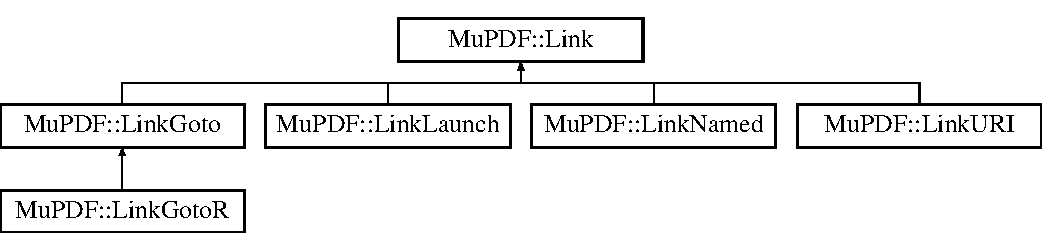
\includegraphics[height=3.000000cm]{class_mu_p_d_f_1_1_link}
\end{center}
\end{figure}
\subsection*{Public Types}
\begin{DoxyCompactItemize}
\item 
enum \hyperlink{class_mu_p_d_f_1_1_link_afdc6828b6e00f323b53d6ae36d0d06b6}{Link\-Type} \{ \\*
\hyperlink{class_mu_p_d_f_1_1_link_afdc6828b6e00f323b53d6ae36d0d06b6a60f06bd9a99b996b6f05f15076814c8e}{None} = 0, 
\hyperlink{class_mu_p_d_f_1_1_link_afdc6828b6e00f323b53d6ae36d0d06b6a8e8dbec5daeb07d386fe261d877639fb}{Goto}, 
\hyperlink{class_mu_p_d_f_1_1_link_afdc6828b6e00f323b53d6ae36d0d06b6af19bc40abcfe48b5816df0cb96ee025f}{U\-R\-I}, 
\hyperlink{class_mu_p_d_f_1_1_link_afdc6828b6e00f323b53d6ae36d0d06b6a2d292d251eaa8666035d5648a24522c8}{Launch}, 
\\*
\hyperlink{class_mu_p_d_f_1_1_link_afdc6828b6e00f323b53d6ae36d0d06b6a64bad01bb17f65698146da642da33983}{Named}, 
\hyperlink{class_mu_p_d_f_1_1_link_afdc6828b6e00f323b53d6ae36d0d06b6a53227a954ff1d67fe8669a282ae68f63}{Goto\-R}
 \}
\end{DoxyCompactItemize}
\subsection*{Public Member Functions}
\begin{DoxyCompactItemize}
\item 
virtual \hyperlink{class_mu_p_d_f_1_1_link_a67672eaaa9b132b64d78079f96f016d7}{$\sim$\-Link} ()
\item 
virtual \hyperlink{class_mu_p_d_f_1_1_link_afdc6828b6e00f323b53d6ae36d0d06b6}{Link\-Type} \hyperlink{class_mu_p_d_f_1_1_link_afe7888c7db760b5a77040cd075911c15}{link\-Type} () const 
\item 
virtual Q\-Rect\-F \hyperlink{class_mu_p_d_f_1_1_link_a09ef952d535704b060e253e869b4c060}{link\-Area} () const 
\begin{DoxyCompactList}\small\item\em Rect area of the link. \end{DoxyCompactList}\end{DoxyCompactItemize}
\subsection*{Protected Member Functions}
\begin{DoxyCompactItemize}
\item 
\hyperlink{class_mu_p_d_f_1_1_link_aafae45b17498aa5b4ddb284563e19bc7}{Link} (Link\-Private $\ast$linkp)
\end{DoxyCompactItemize}
\subsection*{Protected Attributes}
\begin{DoxyCompactItemize}
\item 
Link\-Private $\ast$ \hyperlink{class_mu_p_d_f_1_1_link_a5723c1b46286b89fd7a8fccfa3dc05d2}{d}
\end{DoxyCompactItemize}
\subsection*{Friends}
\begin{DoxyCompactItemize}
\item 
class \hyperlink{class_mu_p_d_f_1_1_link_ab008ed670017e41b6e6bba8707c775d2}{Outline\-Item\-Private}
\end{DoxyCompactItemize}


\subsection{Detailed Description}


Definition at line 12 of file mupdf-\/link.\-h.



\subsection{Member Enumeration Documentation}
\hypertarget{class_mu_p_d_f_1_1_link_afdc6828b6e00f323b53d6ae36d0d06b6}{\index{Mu\-P\-D\-F\-::\-Link@{Mu\-P\-D\-F\-::\-Link}!Link\-Type@{Link\-Type}}
\index{Link\-Type@{Link\-Type}!MuPDF::Link@{Mu\-P\-D\-F\-::\-Link}}
\subsubsection[{Link\-Type}]{\setlength{\rightskip}{0pt plus 5cm}enum {\bf Mu\-P\-D\-F\-::\-Link\-::\-Link\-Type}}}\label{class_mu_p_d_f_1_1_link_afdc6828b6e00f323b53d6ae36d0d06b6}
\begin{Desc}
\item[Enumerator]\par
\begin{description}
\index{None@{None}!Mu\-P\-D\-F\-::\-Link@{Mu\-P\-D\-F\-::\-Link}}\index{Mu\-P\-D\-F\-::\-Link@{Mu\-P\-D\-F\-::\-Link}!None@{None}}\item[{\em 
\hypertarget{class_mu_p_d_f_1_1_link_afdc6828b6e00f323b53d6ae36d0d06b6a60f06bd9a99b996b6f05f15076814c8e}{None}\label{class_mu_p_d_f_1_1_link_afdc6828b6e00f323b53d6ae36d0d06b6a60f06bd9a99b996b6f05f15076814c8e}
}]\index{Goto@{Goto}!Mu\-P\-D\-F\-::\-Link@{Mu\-P\-D\-F\-::\-Link}}\index{Mu\-P\-D\-F\-::\-Link@{Mu\-P\-D\-F\-::\-Link}!Goto@{Goto}}\item[{\em 
\hypertarget{class_mu_p_d_f_1_1_link_afdc6828b6e00f323b53d6ae36d0d06b6a8e8dbec5daeb07d386fe261d877639fb}{Goto}\label{class_mu_p_d_f_1_1_link_afdc6828b6e00f323b53d6ae36d0d06b6a8e8dbec5daeb07d386fe261d877639fb}
}]Goto a position in current file. \index{U\-R\-I@{U\-R\-I}!Mu\-P\-D\-F\-::\-Link@{Mu\-P\-D\-F\-::\-Link}}\index{Mu\-P\-D\-F\-::\-Link@{Mu\-P\-D\-F\-::\-Link}!U\-R\-I@{U\-R\-I}}\item[{\em 
\hypertarget{class_mu_p_d_f_1_1_link_afdc6828b6e00f323b53d6ae36d0d06b6af19bc40abcfe48b5816df0cb96ee025f}{U\-R\-I}\label{class_mu_p_d_f_1_1_link_afdc6828b6e00f323b53d6ae36d0d06b6af19bc40abcfe48b5816df0cb96ee025f}
}]A U\-R\-I link. \index{Launch@{Launch}!Mu\-P\-D\-F\-::\-Link@{Mu\-P\-D\-F\-::\-Link}}\index{Mu\-P\-D\-F\-::\-Link@{Mu\-P\-D\-F\-::\-Link}!Launch@{Launch}}\item[{\em 
\hypertarget{class_mu_p_d_f_1_1_link_afdc6828b6e00f323b53d6ae36d0d06b6a2d292d251eaa8666035d5648a24522c8}{Launch}\label{class_mu_p_d_f_1_1_link_afdc6828b6e00f323b53d6ae36d0d06b6a2d292d251eaa8666035d5648a24522c8}
}]Launch a file (a document or a executable) \index{Named@{Named}!Mu\-P\-D\-F\-::\-Link@{Mu\-P\-D\-F\-::\-Link}}\index{Mu\-P\-D\-F\-::\-Link@{Mu\-P\-D\-F\-::\-Link}!Named@{Named}}\item[{\em 
\hypertarget{class_mu_p_d_f_1_1_link_afdc6828b6e00f323b53d6ae36d0d06b6a64bad01bb17f65698146da642da33983}{Named}\label{class_mu_p_d_f_1_1_link_afdc6828b6e00f323b53d6ae36d0d06b6a64bad01bb17f65698146da642da33983}
}]Named action to perform. \index{Goto\-R@{Goto\-R}!Mu\-P\-D\-F\-::\-Link@{Mu\-P\-D\-F\-::\-Link}}\index{Mu\-P\-D\-F\-::\-Link@{Mu\-P\-D\-F\-::\-Link}!Goto\-R@{Goto\-R}}\item[{\em 
\hypertarget{class_mu_p_d_f_1_1_link_afdc6828b6e00f323b53d6ae36d0d06b6a53227a954ff1d67fe8669a282ae68f63}{Goto\-R}\label{class_mu_p_d_f_1_1_link_afdc6828b6e00f323b53d6ae36d0d06b6a53227a954ff1d67fe8669a282ae68f63}
}]Goto a position in another file. \end{description}
\end{Desc}


Definition at line 15 of file mupdf-\/link.\-h.



\subsection{Constructor \& Destructor Documentation}
\hypertarget{class_mu_p_d_f_1_1_link_a67672eaaa9b132b64d78079f96f016d7}{\index{Mu\-P\-D\-F\-::\-Link@{Mu\-P\-D\-F\-::\-Link}!$\sim$\-Link@{$\sim$\-Link}}
\index{$\sim$\-Link@{$\sim$\-Link}!MuPDF::Link@{Mu\-P\-D\-F\-::\-Link}}
\subsubsection[{$\sim$\-Link}]{\setlength{\rightskip}{0pt plus 5cm}Mu\-P\-D\-F\-::\-Link\-::$\sim$\-Link (
\begin{DoxyParamCaption}
{}
\end{DoxyParamCaption}
)\hspace{0.3cm}{\ttfamily [virtual]}}}\label{class_mu_p_d_f_1_1_link_a67672eaaa9b132b64d78079f96f016d7}


Definition at line 12 of file mupdf-\/link.\-cpp.

\hypertarget{class_mu_p_d_f_1_1_link_aafae45b17498aa5b4ddb284563e19bc7}{\index{Mu\-P\-D\-F\-::\-Link@{Mu\-P\-D\-F\-::\-Link}!Link@{Link}}
\index{Link@{Link}!MuPDF::Link@{Mu\-P\-D\-F\-::\-Link}}
\subsubsection[{Link}]{\setlength{\rightskip}{0pt plus 5cm}Mu\-P\-D\-F\-::\-Link\-::\-Link (
\begin{DoxyParamCaption}
\item[{Link\-Private $\ast$}]{linkp}
\end{DoxyParamCaption}
)\hspace{0.3cm}{\ttfamily [inline]}, {\ttfamily [protected]}}}\label{class_mu_p_d_f_1_1_link_aafae45b17498aa5b4ddb284563e19bc7}


Definition at line 31 of file mupdf-\/link.\-h.



\subsection{Member Function Documentation}
\hypertarget{class_mu_p_d_f_1_1_link_a09ef952d535704b060e253e869b4c060}{\index{Mu\-P\-D\-F\-::\-Link@{Mu\-P\-D\-F\-::\-Link}!link\-Area@{link\-Area}}
\index{link\-Area@{link\-Area}!MuPDF::Link@{Mu\-P\-D\-F\-::\-Link}}
\subsubsection[{link\-Area}]{\setlength{\rightskip}{0pt plus 5cm}Q\-Rect\-F Mu\-P\-D\-F\-::\-Link\-::link\-Area (
\begin{DoxyParamCaption}
{}
\end{DoxyParamCaption}
) const\hspace{0.3cm}{\ttfamily [virtual]}}}\label{class_mu_p_d_f_1_1_link_a09ef952d535704b060e253e869b4c060}


Rect area of the link. 



Definition at line 20 of file mupdf-\/link.\-cpp.

\hypertarget{class_mu_p_d_f_1_1_link_afe7888c7db760b5a77040cd075911c15}{\index{Mu\-P\-D\-F\-::\-Link@{Mu\-P\-D\-F\-::\-Link}!link\-Type@{link\-Type}}
\index{link\-Type@{link\-Type}!MuPDF::Link@{Mu\-P\-D\-F\-::\-Link}}
\subsubsection[{link\-Type}]{\setlength{\rightskip}{0pt plus 5cm}virtual {\bf Link\-Type} Mu\-P\-D\-F\-::\-Link\-::link\-Type (
\begin{DoxyParamCaption}
{}
\end{DoxyParamCaption}
) const\hspace{0.3cm}{\ttfamily [inline]}, {\ttfamily [virtual]}}}\label{class_mu_p_d_f_1_1_link_afe7888c7db760b5a77040cd075911c15}


Reimplemented in \hyperlink{class_mu_p_d_f_1_1_link_goto_r_a0528b0bb75308cbad4c1ad6936daa48c}{Mu\-P\-D\-F\-::\-Link\-Goto\-R}, \hyperlink{class_mu_p_d_f_1_1_link_named_af1037fb72e88df68b918b6f46a948ee1}{Mu\-P\-D\-F\-::\-Link\-Named}, \hyperlink{class_mu_p_d_f_1_1_link_launch_aea60c0a000b7ce966097714e83fb68f8}{Mu\-P\-D\-F\-::\-Link\-Launch}, \hyperlink{class_mu_p_d_f_1_1_link_u_r_i_a32a9aea97620ed712100859e877597fe}{Mu\-P\-D\-F\-::\-Link\-U\-R\-I}, and \hyperlink{class_mu_p_d_f_1_1_link_goto_a057e2224fc0495b171d097f5886ae40a}{Mu\-P\-D\-F\-::\-Link\-Goto}.



Definition at line 27 of file mupdf-\/link.\-h.



\subsection{Friends And Related Function Documentation}
\hypertarget{class_mu_p_d_f_1_1_link_ab008ed670017e41b6e6bba8707c775d2}{\index{Mu\-P\-D\-F\-::\-Link@{Mu\-P\-D\-F\-::\-Link}!Outline\-Item\-Private@{Outline\-Item\-Private}}
\index{Outline\-Item\-Private@{Outline\-Item\-Private}!MuPDF::Link@{Mu\-P\-D\-F\-::\-Link}}
\subsubsection[{Outline\-Item\-Private}]{\setlength{\rightskip}{0pt plus 5cm}friend class Outline\-Item\-Private\hspace{0.3cm}{\ttfamily [friend]}}}\label{class_mu_p_d_f_1_1_link_ab008ed670017e41b6e6bba8707c775d2}


Definition at line 35 of file mupdf-\/link.\-h.



\subsection{Member Data Documentation}
\hypertarget{class_mu_p_d_f_1_1_link_a5723c1b46286b89fd7a8fccfa3dc05d2}{\index{Mu\-P\-D\-F\-::\-Link@{Mu\-P\-D\-F\-::\-Link}!d@{d}}
\index{d@{d}!MuPDF::Link@{Mu\-P\-D\-F\-::\-Link}}
\subsubsection[{d}]{\setlength{\rightskip}{0pt plus 5cm}Link\-Private$\ast$ Mu\-P\-D\-F\-::\-Link\-::d\hspace{0.3cm}{\ttfamily [protected]}}}\label{class_mu_p_d_f_1_1_link_a5723c1b46286b89fd7a8fccfa3dc05d2}


Definition at line 33 of file mupdf-\/link.\-h.



The documentation for this class was generated from the following files\-:\begin{DoxyCompactItemize}
\item 
/home/a/project/mupdf-\/qt/include/\hyperlink{mupdf-link_8h}{mupdf-\/link.\-h}\item 
/home/a/project/mupdf-\/qt/src/\hyperlink{mupdf-link_8cpp}{mupdf-\/link.\-cpp}\end{DoxyCompactItemize}

\hypertarget{class_mu_p_d_f_1_1_link_goto}{\section{Mu\-P\-D\-F\-:\-:Link\-Goto Class Reference}
\label{class_mu_p_d_f_1_1_link_goto}\index{Mu\-P\-D\-F\-::\-Link\-Goto@{Mu\-P\-D\-F\-::\-Link\-Goto}}
}


Goto a position in current file.  




{\ttfamily \#include $<$mupdf-\/link.\-h$>$}

Inheritance diagram for Mu\-P\-D\-F\-:\-:Link\-Goto\-:\begin{figure}[H]
\begin{center}
\leavevmode
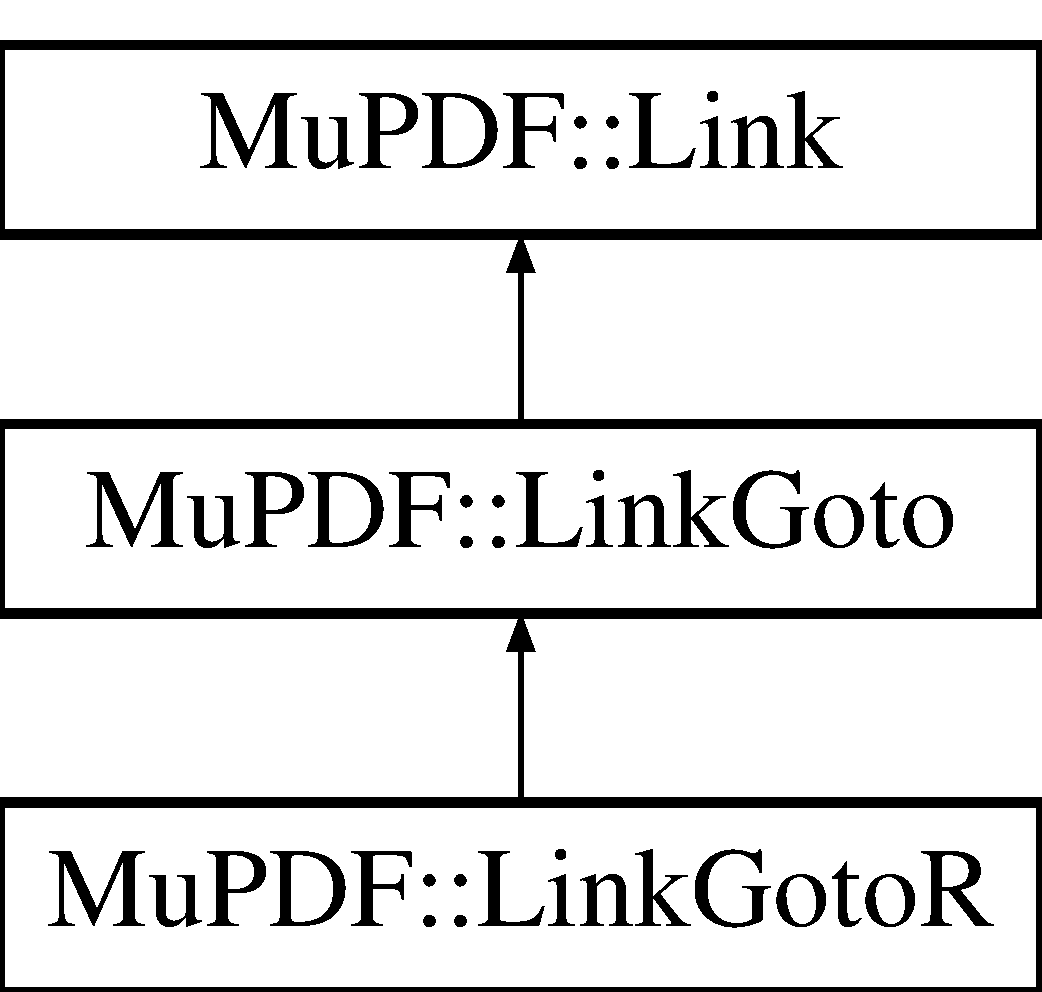
\includegraphics[height=3.000000cm]{class_mu_p_d_f_1_1_link_goto}
\end{center}
\end{figure}
\subsection*{Public Member Functions}
\begin{DoxyCompactItemize}
\item 
\hyperlink{class_mu_p_d_f_1_1_link_afdc6828b6e00f323b53d6ae36d0d06b6}{Link\-Type} \hyperlink{class_mu_p_d_f_1_1_link_goto_a057e2224fc0495b171d097f5886ae40a}{link\-Type} () const 
\item 
int \hyperlink{class_mu_p_d_f_1_1_link_goto_a83be7a158c0d4a3f8d61bfd0c3413d8c}{page} () const 
\begin{DoxyCompactList}\small\item\em \hyperlink{class_mu_p_d_f_1_1_page}{Page} number(start from 0). \end{DoxyCompactList}\item 
bool \hyperlink{class_mu_p_d_f_1_1_link_goto_a7074767dce7801874821840faa844917}{fit\-Horizontally} () const 
\begin{DoxyCompactList}\small\item\em Fit horizontally. \end{DoxyCompactList}\item 
bool \hyperlink{class_mu_p_d_f_1_1_link_goto_aea9a77cf7b01a2fc170afe35d7452c87}{fit\-Vertically} () const 
\begin{DoxyCompactList}\small\item\em Fit vertically. \end{DoxyCompactList}\item 
float \hyperlink{class_mu_p_d_f_1_1_link_goto_ab13b98ecc306c81149347eb05acbbcc1}{zoom} () const 
\begin{DoxyCompactList}\small\item\em Zoom ratio. \end{DoxyCompactList}\end{DoxyCompactItemize}
\subsection*{Protected Member Functions}
\begin{DoxyCompactItemize}
\item 
\hyperlink{class_mu_p_d_f_1_1_link_goto_a2e6b496f89b8aa6162e558f9536d4dbc}{Link\-Goto} (Link\-Private $\ast$linkp)
\end{DoxyCompactItemize}
\subsection*{Friends}
\begin{DoxyCompactItemize}
\item 
class \hyperlink{class_mu_p_d_f_1_1_link_goto_ab008ed670017e41b6e6bba8707c775d2}{Outline\-Item\-Private}
\end{DoxyCompactItemize}
\subsection*{Additional Inherited Members}


\subsection{Detailed Description}
Goto a position in current file. 

Definition at line 41 of file mupdf-\/link.\-h.



\subsection{Constructor \& Destructor Documentation}
\hypertarget{class_mu_p_d_f_1_1_link_goto_a2e6b496f89b8aa6162e558f9536d4dbc}{\index{Mu\-P\-D\-F\-::\-Link\-Goto@{Mu\-P\-D\-F\-::\-Link\-Goto}!Link\-Goto@{Link\-Goto}}
\index{Link\-Goto@{Link\-Goto}!MuPDF::LinkGoto@{Mu\-P\-D\-F\-::\-Link\-Goto}}
\subsubsection[{Link\-Goto}]{\setlength{\rightskip}{0pt plus 5cm}Mu\-P\-D\-F\-::\-Link\-Goto\-::\-Link\-Goto (
\begin{DoxyParamCaption}
\item[{Link\-Private $\ast$}]{linkp}
\end{DoxyParamCaption}
)\hspace{0.3cm}{\ttfamily [inline]}, {\ttfamily [protected]}}}\label{class_mu_p_d_f_1_1_link_goto_a2e6b496f89b8aa6162e558f9536d4dbc}


Definition at line 51 of file mupdf-\/link.\-h.



\subsection{Member Function Documentation}
\hypertarget{class_mu_p_d_f_1_1_link_goto_a7074767dce7801874821840faa844917}{\index{Mu\-P\-D\-F\-::\-Link\-Goto@{Mu\-P\-D\-F\-::\-Link\-Goto}!fit\-Horizontally@{fit\-Horizontally}}
\index{fit\-Horizontally@{fit\-Horizontally}!MuPDF::LinkGoto@{Mu\-P\-D\-F\-::\-Link\-Goto}}
\subsubsection[{fit\-Horizontally}]{\setlength{\rightskip}{0pt plus 5cm}bool Mu\-P\-D\-F\-::\-Link\-Goto\-::fit\-Horizontally (
\begin{DoxyParamCaption}
{}
\end{DoxyParamCaption}
) const}}\label{class_mu_p_d_f_1_1_link_goto_a7074767dce7801874821840faa844917}


Fit horizontally. 



Definition at line 37 of file mupdf-\/link.\-cpp.

\hypertarget{class_mu_p_d_f_1_1_link_goto_aea9a77cf7b01a2fc170afe35d7452c87}{\index{Mu\-P\-D\-F\-::\-Link\-Goto@{Mu\-P\-D\-F\-::\-Link\-Goto}!fit\-Vertically@{fit\-Vertically}}
\index{fit\-Vertically@{fit\-Vertically}!MuPDF::LinkGoto@{Mu\-P\-D\-F\-::\-Link\-Goto}}
\subsubsection[{fit\-Vertically}]{\setlength{\rightskip}{0pt plus 5cm}bool Mu\-P\-D\-F\-::\-Link\-Goto\-::fit\-Vertically (
\begin{DoxyParamCaption}
{}
\end{DoxyParamCaption}
) const}}\label{class_mu_p_d_f_1_1_link_goto_aea9a77cf7b01a2fc170afe35d7452c87}


Fit vertically. 



Definition at line 45 of file mupdf-\/link.\-cpp.

\hypertarget{class_mu_p_d_f_1_1_link_goto_a057e2224fc0495b171d097f5886ae40a}{\index{Mu\-P\-D\-F\-::\-Link\-Goto@{Mu\-P\-D\-F\-::\-Link\-Goto}!link\-Type@{link\-Type}}
\index{link\-Type@{link\-Type}!MuPDF::LinkGoto@{Mu\-P\-D\-F\-::\-Link\-Goto}}
\subsubsection[{link\-Type}]{\setlength{\rightskip}{0pt plus 5cm}{\bf Link\-Type} Mu\-P\-D\-F\-::\-Link\-Goto\-::link\-Type (
\begin{DoxyParamCaption}
{}
\end{DoxyParamCaption}
) const\hspace{0.3cm}{\ttfamily [inline]}, {\ttfamily [virtual]}}}\label{class_mu_p_d_f_1_1_link_goto_a057e2224fc0495b171d097f5886ae40a}


Reimplemented from \hyperlink{class_mu_p_d_f_1_1_link_afe7888c7db760b5a77040cd075911c15}{Mu\-P\-D\-F\-::\-Link}.



Reimplemented in \hyperlink{class_mu_p_d_f_1_1_link_goto_r_a0528b0bb75308cbad4c1ad6936daa48c}{Mu\-P\-D\-F\-::\-Link\-Goto\-R}.



Definition at line 44 of file mupdf-\/link.\-h.

\hypertarget{class_mu_p_d_f_1_1_link_goto_a83be7a158c0d4a3f8d61bfd0c3413d8c}{\index{Mu\-P\-D\-F\-::\-Link\-Goto@{Mu\-P\-D\-F\-::\-Link\-Goto}!page@{page}}
\index{page@{page}!MuPDF::LinkGoto@{Mu\-P\-D\-F\-::\-Link\-Goto}}
\subsubsection[{page}]{\setlength{\rightskip}{0pt plus 5cm}int Mu\-P\-D\-F\-::\-Link\-Goto\-::page (
\begin{DoxyParamCaption}
{}
\end{DoxyParamCaption}
) const}}\label{class_mu_p_d_f_1_1_link_goto_a83be7a158c0d4a3f8d61bfd0c3413d8c}


\hyperlink{class_mu_p_d_f_1_1_page}{Page} number(start from 0). 



Definition at line 29 of file mupdf-\/link.\-cpp.

\hypertarget{class_mu_p_d_f_1_1_link_goto_ab13b98ecc306c81149347eb05acbbcc1}{\index{Mu\-P\-D\-F\-::\-Link\-Goto@{Mu\-P\-D\-F\-::\-Link\-Goto}!zoom@{zoom}}
\index{zoom@{zoom}!MuPDF::LinkGoto@{Mu\-P\-D\-F\-::\-Link\-Goto}}
\subsubsection[{zoom}]{\setlength{\rightskip}{0pt plus 5cm}float Mu\-P\-D\-F\-::\-Link\-Goto\-::zoom (
\begin{DoxyParamCaption}
{}
\end{DoxyParamCaption}
) const}}\label{class_mu_p_d_f_1_1_link_goto_ab13b98ecc306c81149347eb05acbbcc1}


Zoom ratio. 

\begin{DoxyReturn}{Returns}
Do not change zoom ratio when 0.\-0f is returned. 
\end{DoxyReturn}


Definition at line 55 of file mupdf-\/link.\-cpp.



\subsection{Friends And Related Function Documentation}
\hypertarget{class_mu_p_d_f_1_1_link_goto_ab008ed670017e41b6e6bba8707c775d2}{\index{Mu\-P\-D\-F\-::\-Link\-Goto@{Mu\-P\-D\-F\-::\-Link\-Goto}!Outline\-Item\-Private@{Outline\-Item\-Private}}
\index{Outline\-Item\-Private@{Outline\-Item\-Private}!MuPDF::LinkGoto@{Mu\-P\-D\-F\-::\-Link\-Goto}}
\subsubsection[{Outline\-Item\-Private}]{\setlength{\rightskip}{0pt plus 5cm}friend class Outline\-Item\-Private\hspace{0.3cm}{\ttfamily [friend]}}}\label{class_mu_p_d_f_1_1_link_goto_ab008ed670017e41b6e6bba8707c775d2}


Definition at line 53 of file mupdf-\/link.\-h.



The documentation for this class was generated from the following files\-:\begin{DoxyCompactItemize}
\item 
/home/a/project/mupdf-\/qt/include/\hyperlink{mupdf-link_8h}{mupdf-\/link.\-h}\item 
/home/a/project/mupdf-\/qt/src/\hyperlink{mupdf-link_8cpp}{mupdf-\/link.\-cpp}\end{DoxyCompactItemize}

\hypertarget{class_mu_p_d_f_1_1_link_goto_r}{\section{Mu\-P\-D\-F\-:\-:Link\-Goto\-R Class Reference}
\label{class_mu_p_d_f_1_1_link_goto_r}\index{Mu\-P\-D\-F\-::\-Link\-Goto\-R@{Mu\-P\-D\-F\-::\-Link\-Goto\-R}}
}


Goto a position in another file.  




{\ttfamily \#include $<$mupdf-\/link.\-h$>$}

Inheritance diagram for Mu\-P\-D\-F\-:\-:Link\-Goto\-R\-:\begin{figure}[H]
\begin{center}
\leavevmode
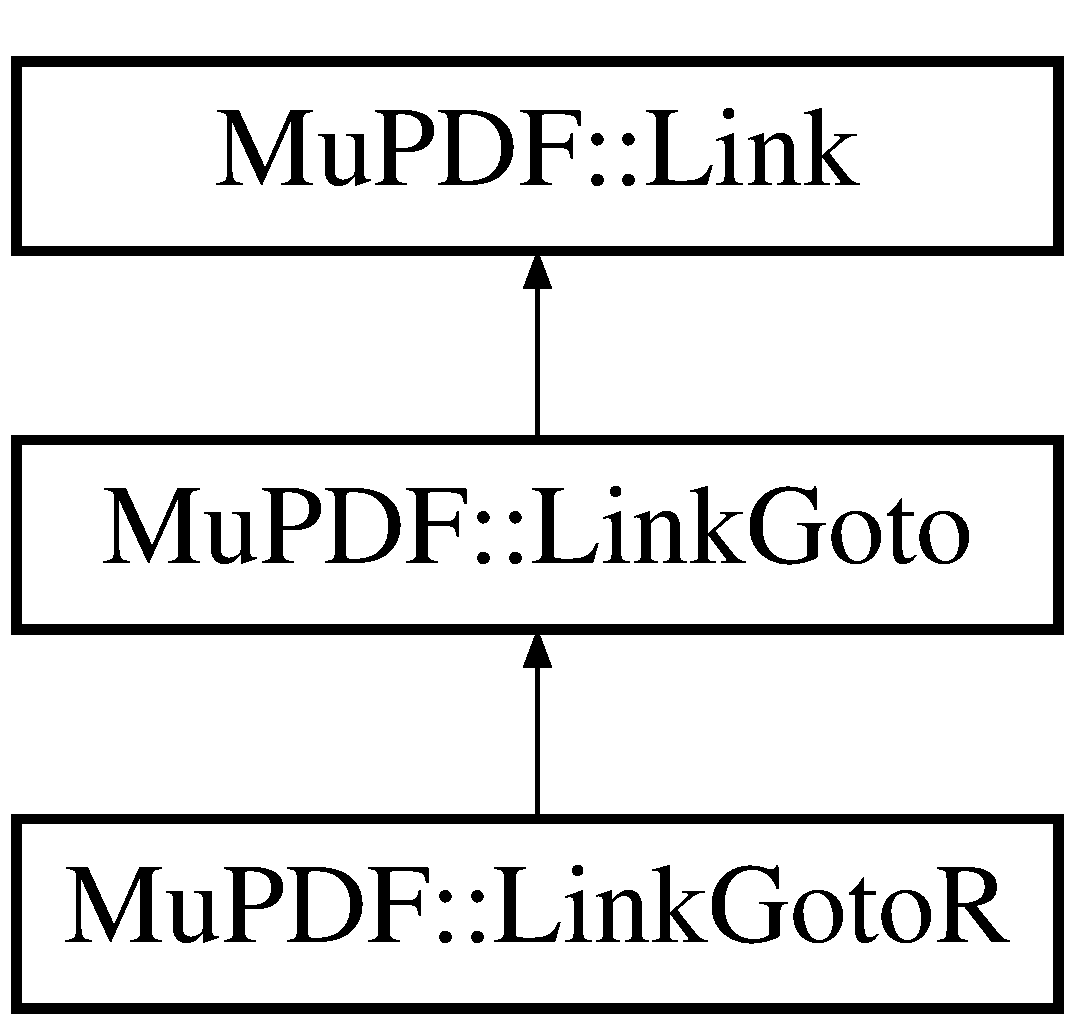
\includegraphics[height=3.000000cm]{class_mu_p_d_f_1_1_link_goto_r}
\end{center}
\end{figure}
\subsection*{Public Member Functions}
\begin{DoxyCompactItemize}
\item 
\hyperlink{class_mu_p_d_f_1_1_link_afdc6828b6e00f323b53d6ae36d0d06b6}{Link\-Type} \hyperlink{class_mu_p_d_f_1_1_link_goto_r_a0528b0bb75308cbad4c1ad6936daa48c}{link\-Type} () const 
\item 
int \hyperlink{class_mu_p_d_f_1_1_link_goto_r_a506a78720f51b9928517273c63470a81}{page} () const 
\begin{DoxyCompactList}\small\item\em \hyperlink{class_mu_p_d_f_1_1_page}{Page} number(start from 0). \end{DoxyCompactList}\item 
Q\-String \hyperlink{class_mu_p_d_f_1_1_link_goto_r_ab5ff953c35930b5ff57740decee8c61b}{destination} () const 
\begin{DoxyCompactList}\small\item\em The target destination name to be resolved in the \hyperlink{class_mu_p_d_f_1_1_link_goto_r_aeef07c41fa5450bf6358406011402ccd}{file()}. \end{DoxyCompactList}\item 
Q\-String \hyperlink{class_mu_p_d_f_1_1_link_goto_r_aeef07c41fa5450bf6358406011402ccd}{file} () const 
\begin{DoxyCompactList}\small\item\em A pointer to a remote file specification (U\-T\-F-\/8). If set, this destination should cause a new file to be opened. \end{DoxyCompactList}\item 
bool \hyperlink{class_mu_p_d_f_1_1_link_goto_r_a588e406a62ba86fffcc907f890342196}{new\-Window} () const 
\begin{DoxyCompactList}\small\item\em If true, the destination should open in a new window. \end{DoxyCompactList}\end{DoxyCompactItemize}
\subsection*{Friends}
\begin{DoxyCompactItemize}
\item 
class \hyperlink{class_mu_p_d_f_1_1_link_goto_r_ab008ed670017e41b6e6bba8707c775d2}{Outline\-Item\-Private}
\end{DoxyCompactItemize}
\subsection*{Additional Inherited Members}


\subsection{Detailed Description}
Goto a position in another file. 

Definition at line 107 of file mupdf-\/link.\-h.



\subsection{Member Function Documentation}
\hypertarget{class_mu_p_d_f_1_1_link_goto_r_ab5ff953c35930b5ff57740decee8c61b}{\index{Mu\-P\-D\-F\-::\-Link\-Goto\-R@{Mu\-P\-D\-F\-::\-Link\-Goto\-R}!destination@{destination}}
\index{destination@{destination}!MuPDF::LinkGotoR@{Mu\-P\-D\-F\-::\-Link\-Goto\-R}}
\subsubsection[{destination}]{\setlength{\rightskip}{0pt plus 5cm}Q\-String Mu\-P\-D\-F\-::\-Link\-Goto\-R\-::destination (
\begin{DoxyParamCaption}
{}
\end{DoxyParamCaption}
) const}}\label{class_mu_p_d_f_1_1_link_goto_r_ab5ff953c35930b5ff57740decee8c61b}


The target destination name to be resolved in the \hyperlink{class_mu_p_d_f_1_1_link_goto_r_aeef07c41fa5450bf6358406011402ccd}{file()}. 

\begin{DoxyReturn}{Returns}
Maybe empty. 
\end{DoxyReturn}


Definition at line 128 of file mupdf-\/link.\-cpp.

\hypertarget{class_mu_p_d_f_1_1_link_goto_r_aeef07c41fa5450bf6358406011402ccd}{\index{Mu\-P\-D\-F\-::\-Link\-Goto\-R@{Mu\-P\-D\-F\-::\-Link\-Goto\-R}!file@{file}}
\index{file@{file}!MuPDF::LinkGotoR@{Mu\-P\-D\-F\-::\-Link\-Goto\-R}}
\subsubsection[{file}]{\setlength{\rightskip}{0pt plus 5cm}Q\-String Mu\-P\-D\-F\-::\-Link\-Goto\-R\-::file (
\begin{DoxyParamCaption}
{}
\end{DoxyParamCaption}
) const}}\label{class_mu_p_d_f_1_1_link_goto_r_aeef07c41fa5450bf6358406011402ccd}


A pointer to a remote file specification (U\-T\-F-\/8). If set, this destination should cause a new file to be opened. 



Definition at line 137 of file mupdf-\/link.\-cpp.

\hypertarget{class_mu_p_d_f_1_1_link_goto_r_a0528b0bb75308cbad4c1ad6936daa48c}{\index{Mu\-P\-D\-F\-::\-Link\-Goto\-R@{Mu\-P\-D\-F\-::\-Link\-Goto\-R}!link\-Type@{link\-Type}}
\index{link\-Type@{link\-Type}!MuPDF::LinkGotoR@{Mu\-P\-D\-F\-::\-Link\-Goto\-R}}
\subsubsection[{link\-Type}]{\setlength{\rightskip}{0pt plus 5cm}{\bf Link\-Type} Mu\-P\-D\-F\-::\-Link\-Goto\-R\-::link\-Type (
\begin{DoxyParamCaption}
{}
\end{DoxyParamCaption}
) const\hspace{0.3cm}{\ttfamily [inline]}, {\ttfamily [virtual]}}}\label{class_mu_p_d_f_1_1_link_goto_r_a0528b0bb75308cbad4c1ad6936daa48c}


Reimplemented from \hyperlink{class_mu_p_d_f_1_1_link_goto_a057e2224fc0495b171d097f5886ae40a}{Mu\-P\-D\-F\-::\-Link\-Goto}.



Definition at line 110 of file mupdf-\/link.\-h.

\hypertarget{class_mu_p_d_f_1_1_link_goto_r_a588e406a62ba86fffcc907f890342196}{\index{Mu\-P\-D\-F\-::\-Link\-Goto\-R@{Mu\-P\-D\-F\-::\-Link\-Goto\-R}!new\-Window@{new\-Window}}
\index{new\-Window@{new\-Window}!MuPDF::LinkGotoR@{Mu\-P\-D\-F\-::\-Link\-Goto\-R}}
\subsubsection[{new\-Window}]{\setlength{\rightskip}{0pt plus 5cm}bool Mu\-P\-D\-F\-::\-Link\-Goto\-R\-::new\-Window (
\begin{DoxyParamCaption}
{}
\end{DoxyParamCaption}
) const}}\label{class_mu_p_d_f_1_1_link_goto_r_a588e406a62ba86fffcc907f890342196}


If true, the destination should open in a new window. 



Definition at line 145 of file mupdf-\/link.\-cpp.

\hypertarget{class_mu_p_d_f_1_1_link_goto_r_a506a78720f51b9928517273c63470a81}{\index{Mu\-P\-D\-F\-::\-Link\-Goto\-R@{Mu\-P\-D\-F\-::\-Link\-Goto\-R}!page@{page}}
\index{page@{page}!MuPDF::LinkGotoR@{Mu\-P\-D\-F\-::\-Link\-Goto\-R}}
\subsubsection[{page}]{\setlength{\rightskip}{0pt plus 5cm}int Mu\-P\-D\-F\-::\-Link\-Goto\-R\-::page (
\begin{DoxyParamCaption}
{}
\end{DoxyParamCaption}
) const}}\label{class_mu_p_d_f_1_1_link_goto_r_a506a78720f51b9928517273c63470a81}


\hyperlink{class_mu_p_d_f_1_1_page}{Page} number(start from 0). 

\begin{DoxyReturn}{Returns}
-\/1 suggesting that destination is given by \hyperlink{class_mu_p_d_f_1_1_link_goto_r_ab5ff953c35930b5ff57740decee8c61b}{destination()}. 
\end{DoxyReturn}


Definition at line 118 of file mupdf-\/link.\-cpp.



\subsection{Friends And Related Function Documentation}
\hypertarget{class_mu_p_d_f_1_1_link_goto_r_ab008ed670017e41b6e6bba8707c775d2}{\index{Mu\-P\-D\-F\-::\-Link\-Goto\-R@{Mu\-P\-D\-F\-::\-Link\-Goto\-R}!Outline\-Item\-Private@{Outline\-Item\-Private}}
\index{Outline\-Item\-Private@{Outline\-Item\-Private}!MuPDF::LinkGotoR@{Mu\-P\-D\-F\-::\-Link\-Goto\-R}}
\subsubsection[{Outline\-Item\-Private}]{\setlength{\rightskip}{0pt plus 5cm}friend class Outline\-Item\-Private\hspace{0.3cm}{\ttfamily [friend]}}}\label{class_mu_p_d_f_1_1_link_goto_r_ab008ed670017e41b6e6bba8707c775d2}


Definition at line 119 of file mupdf-\/link.\-h.



The documentation for this class was generated from the following files\-:\begin{DoxyCompactItemize}
\item 
/home/a/project/mupdf-\/qt/include/\hyperlink{mupdf-link_8h}{mupdf-\/link.\-h}\item 
/home/a/project/mupdf-\/qt/src/\hyperlink{mupdf-link_8cpp}{mupdf-\/link.\-cpp}\end{DoxyCompactItemize}

\hypertarget{class_mu_p_d_f_1_1_link_launch}{\section{Mu\-P\-D\-F\-:\-:Link\-Launch Class Reference}
\label{class_mu_p_d_f_1_1_link_launch}\index{Mu\-P\-D\-F\-::\-Link\-Launch@{Mu\-P\-D\-F\-::\-Link\-Launch}}
}


Launch a file (a document or a executable).  




{\ttfamily \#include $<$mupdf-\/link.\-h$>$}

Inheritance diagram for Mu\-P\-D\-F\-:\-:Link\-Launch\-:\begin{figure}[H]
\begin{center}
\leavevmode
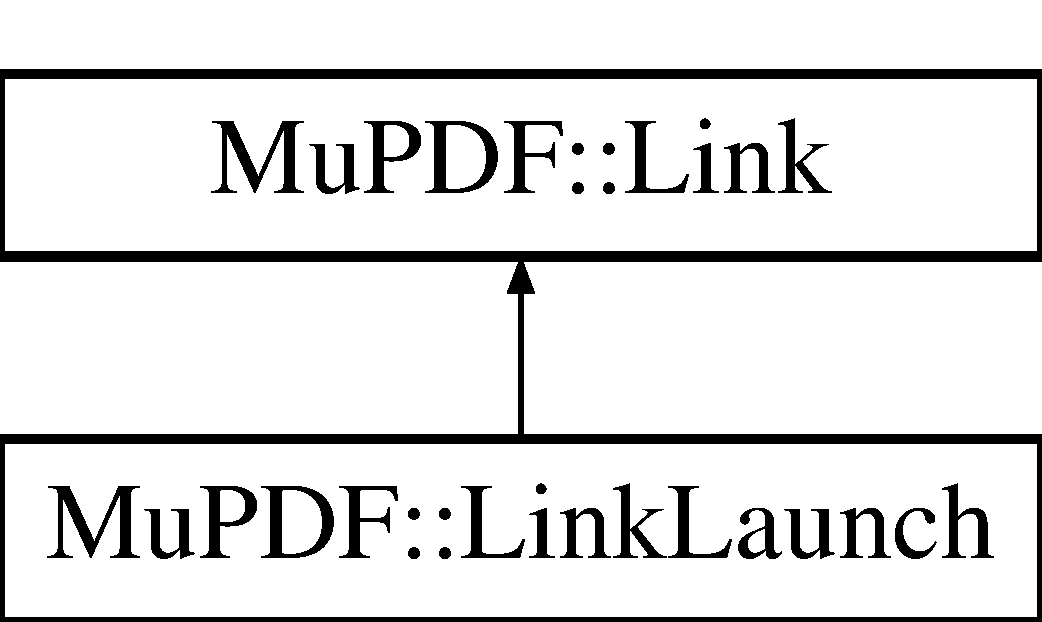
\includegraphics[height=2.000000cm]{class_mu_p_d_f_1_1_link_launch}
\end{center}
\end{figure}
\subsection*{Public Member Functions}
\begin{DoxyCompactItemize}
\item 
\hyperlink{class_mu_p_d_f_1_1_link_afdc6828b6e00f323b53d6ae36d0d06b6}{Link\-Type} \hyperlink{class_mu_p_d_f_1_1_link_launch_aea60c0a000b7ce966097714e83fb68f8}{link\-Type} () const 
\item 
Q\-String \hyperlink{class_mu_p_d_f_1_1_link_launch_ac4d98cbbaa2410b69283cc3d9cbe683b}{file} () const 
\begin{DoxyCompactList}\small\item\em A U\-T\-F-\/8 file specification to launch. \end{DoxyCompactList}\item 
bool \hyperlink{class_mu_p_d_f_1_1_link_launch_a87b88518e72c8018837c18e7ff59d932}{new\-Window} () const 
\begin{DoxyCompactList}\small\item\em If true, the destination should be launched in a new window. \end{DoxyCompactList}\item 
bool \hyperlink{class_mu_p_d_f_1_1_link_launch_a21a4befd2aa791d756187df3d1dc034c}{is\-U\-R\-I} () const 
\begin{DoxyCompactList}\small\item\em If true, \hyperlink{class_mu_p_d_f_1_1_link_launch_ac4d98cbbaa2410b69283cc3d9cbe683b}{file()} is a U\-R\-I to launch. \end{DoxyCompactList}\end{DoxyCompactItemize}
\subsection*{Friends}
\begin{DoxyCompactItemize}
\item 
class \hyperlink{class_mu_p_d_f_1_1_link_launch_ab008ed670017e41b6e6bba8707c775d2}{Outline\-Item\-Private}
\end{DoxyCompactItemize}
\subsection*{Additional Inherited Members}


\subsection{Detailed Description}
Launch a file (a document or a executable). 

Definition at line 75 of file mupdf-\/link.\-h.



\subsection{Member Function Documentation}
\hypertarget{class_mu_p_d_f_1_1_link_launch_ac4d98cbbaa2410b69283cc3d9cbe683b}{\index{Mu\-P\-D\-F\-::\-Link\-Launch@{Mu\-P\-D\-F\-::\-Link\-Launch}!file@{file}}
\index{file@{file}!MuPDF::LinkLaunch@{Mu\-P\-D\-F\-::\-Link\-Launch}}
\subsubsection[{file}]{\setlength{\rightskip}{0pt plus 5cm}Q\-String Mu\-P\-D\-F\-::\-Link\-Launch\-::file (
\begin{DoxyParamCaption}
{}
\end{DoxyParamCaption}
) const}}\label{class_mu_p_d_f_1_1_link_launch_ac4d98cbbaa2410b69283cc3d9cbe683b}


A U\-T\-F-\/8 file specification to launch. 



Definition at line 84 of file mupdf-\/link.\-cpp.

\hypertarget{class_mu_p_d_f_1_1_link_launch_a21a4befd2aa791d756187df3d1dc034c}{\index{Mu\-P\-D\-F\-::\-Link\-Launch@{Mu\-P\-D\-F\-::\-Link\-Launch}!is\-U\-R\-I@{is\-U\-R\-I}}
\index{is\-U\-R\-I@{is\-U\-R\-I}!MuPDF::LinkLaunch@{Mu\-P\-D\-F\-::\-Link\-Launch}}
\subsubsection[{is\-U\-R\-I}]{\setlength{\rightskip}{0pt plus 5cm}bool Mu\-P\-D\-F\-::\-Link\-Launch\-::is\-U\-R\-I (
\begin{DoxyParamCaption}
{}
\end{DoxyParamCaption}
) const}}\label{class_mu_p_d_f_1_1_link_launch_a21a4befd2aa791d756187df3d1dc034c}


If true, \hyperlink{class_mu_p_d_f_1_1_link_launch_ac4d98cbbaa2410b69283cc3d9cbe683b}{file()} is a U\-R\-I to launch. 



Definition at line 100 of file mupdf-\/link.\-cpp.

\hypertarget{class_mu_p_d_f_1_1_link_launch_aea60c0a000b7ce966097714e83fb68f8}{\index{Mu\-P\-D\-F\-::\-Link\-Launch@{Mu\-P\-D\-F\-::\-Link\-Launch}!link\-Type@{link\-Type}}
\index{link\-Type@{link\-Type}!MuPDF::LinkLaunch@{Mu\-P\-D\-F\-::\-Link\-Launch}}
\subsubsection[{link\-Type}]{\setlength{\rightskip}{0pt plus 5cm}{\bf Link\-Type} Mu\-P\-D\-F\-::\-Link\-Launch\-::link\-Type (
\begin{DoxyParamCaption}
{}
\end{DoxyParamCaption}
) const\hspace{0.3cm}{\ttfamily [inline]}, {\ttfamily [virtual]}}}\label{class_mu_p_d_f_1_1_link_launch_aea60c0a000b7ce966097714e83fb68f8}


Reimplemented from \hyperlink{class_mu_p_d_f_1_1_link_afe7888c7db760b5a77040cd075911c15}{Mu\-P\-D\-F\-::\-Link}.



Definition at line 78 of file mupdf-\/link.\-h.

\hypertarget{class_mu_p_d_f_1_1_link_launch_a87b88518e72c8018837c18e7ff59d932}{\index{Mu\-P\-D\-F\-::\-Link\-Launch@{Mu\-P\-D\-F\-::\-Link\-Launch}!new\-Window@{new\-Window}}
\index{new\-Window@{new\-Window}!MuPDF::LinkLaunch@{Mu\-P\-D\-F\-::\-Link\-Launch}}
\subsubsection[{new\-Window}]{\setlength{\rightskip}{0pt plus 5cm}bool Mu\-P\-D\-F\-::\-Link\-Launch\-::new\-Window (
\begin{DoxyParamCaption}
{}
\end{DoxyParamCaption}
) const}}\label{class_mu_p_d_f_1_1_link_launch_a87b88518e72c8018837c18e7ff59d932}


If true, the destination should be launched in a new window. 



Definition at line 92 of file mupdf-\/link.\-cpp.



\subsection{Friends And Related Function Documentation}
\hypertarget{class_mu_p_d_f_1_1_link_launch_ab008ed670017e41b6e6bba8707c775d2}{\index{Mu\-P\-D\-F\-::\-Link\-Launch@{Mu\-P\-D\-F\-::\-Link\-Launch}!Outline\-Item\-Private@{Outline\-Item\-Private}}
\index{Outline\-Item\-Private@{Outline\-Item\-Private}!MuPDF::LinkLaunch@{Mu\-P\-D\-F\-::\-Link\-Launch}}
\subsubsection[{Outline\-Item\-Private}]{\setlength{\rightskip}{0pt plus 5cm}friend class Outline\-Item\-Private\hspace{0.3cm}{\ttfamily [friend]}}}\label{class_mu_p_d_f_1_1_link_launch_ab008ed670017e41b6e6bba8707c775d2}


Definition at line 86 of file mupdf-\/link.\-h.



The documentation for this class was generated from the following files\-:\begin{DoxyCompactItemize}
\item 
libmupdf-\/qt/\hyperlink{mupdf-link_8h}{mupdf-\/link.\-h}\item 
libmupdf-\/qt/\hyperlink{mupdf-link_8cpp}{mupdf-\/link.\-cpp}\end{DoxyCompactItemize}

\hypertarget{class_mu_p_d_f_1_1_link_named}{\section{Mu\-P\-D\-F\-:\-:Link\-Named Class Reference}
\label{class_mu_p_d_f_1_1_link_named}\index{Mu\-P\-D\-F\-::\-Link\-Named@{Mu\-P\-D\-F\-::\-Link\-Named}}
}


Named action to perform.  




{\ttfamily \#include $<$mupdf-\/link.\-h$>$}

Inheritance diagram for Mu\-P\-D\-F\-:\-:Link\-Named\-:\begin{figure}[H]
\begin{center}
\leavevmode
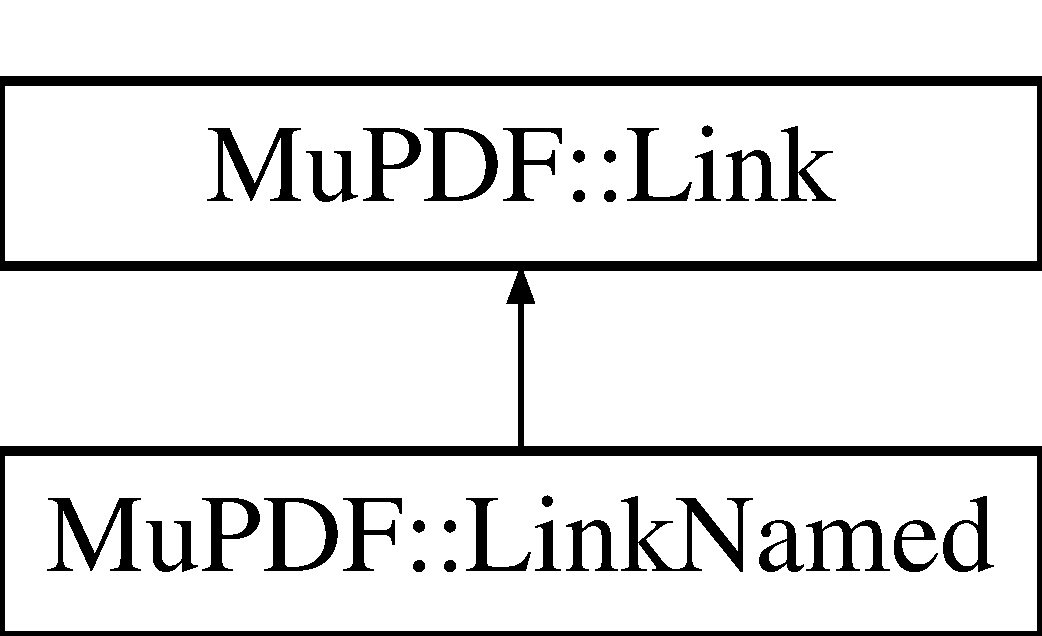
\includegraphics[height=2.000000cm]{class_mu_p_d_f_1_1_link_named}
\end{center}
\end{figure}
\subsection*{Public Member Functions}
\begin{DoxyCompactItemize}
\item 
\hyperlink{class_mu_p_d_f_1_1_link_afdc6828b6e00f323b53d6ae36d0d06b6}{Link\-Type} \hyperlink{class_mu_p_d_f_1_1_link_named_af1037fb72e88df68b918b6f46a948ee1}{link\-Type} () const 
\item 
Q\-String \hyperlink{class_mu_p_d_f_1_1_link_named_a6573eed025194f585407d97373359595}{named} () const 
\begin{DoxyCompactList}\small\item\em The named action to perform. \end{DoxyCompactList}\end{DoxyCompactItemize}
\subsection*{Friends}
\begin{DoxyCompactItemize}
\item 
class \hyperlink{class_mu_p_d_f_1_1_link_named_ab008ed670017e41b6e6bba8707c775d2}{Outline\-Item\-Private}
\end{DoxyCompactItemize}
\subsection*{Additional Inherited Members}


\subsection{Detailed Description}
Named action to perform. 

Definition at line 92 of file mupdf-\/link.\-h.



\subsection{Member Function Documentation}
\hypertarget{class_mu_p_d_f_1_1_link_named_af1037fb72e88df68b918b6f46a948ee1}{\index{Mu\-P\-D\-F\-::\-Link\-Named@{Mu\-P\-D\-F\-::\-Link\-Named}!link\-Type@{link\-Type}}
\index{link\-Type@{link\-Type}!MuPDF::LinkNamed@{Mu\-P\-D\-F\-::\-Link\-Named}}
\subsubsection[{link\-Type}]{\setlength{\rightskip}{0pt plus 5cm}{\bf Link\-Type} Mu\-P\-D\-F\-::\-Link\-Named\-::link\-Type (
\begin{DoxyParamCaption}
{}
\end{DoxyParamCaption}
) const\hspace{0.3cm}{\ttfamily [inline]}, {\ttfamily [virtual]}}}\label{class_mu_p_d_f_1_1_link_named_af1037fb72e88df68b918b6f46a948ee1}


Reimplemented from \hyperlink{class_mu_p_d_f_1_1_link_afe7888c7db760b5a77040cd075911c15}{Mu\-P\-D\-F\-::\-Link}.



Definition at line 95 of file mupdf-\/link.\-h.

\hypertarget{class_mu_p_d_f_1_1_link_named_a6573eed025194f585407d97373359595}{\index{Mu\-P\-D\-F\-::\-Link\-Named@{Mu\-P\-D\-F\-::\-Link\-Named}!named@{named}}
\index{named@{named}!MuPDF::LinkNamed@{Mu\-P\-D\-F\-::\-Link\-Named}}
\subsubsection[{named}]{\setlength{\rightskip}{0pt plus 5cm}Q\-String Mu\-P\-D\-F\-::\-Link\-Named\-::named (
\begin{DoxyParamCaption}
{}
\end{DoxyParamCaption}
) const}}\label{class_mu_p_d_f_1_1_link_named_a6573eed025194f585407d97373359595}


The named action to perform. 



Definition at line 108 of file mupdf-\/link.\-cpp.



\subsection{Friends And Related Function Documentation}
\hypertarget{class_mu_p_d_f_1_1_link_named_ab008ed670017e41b6e6bba8707c775d2}{\index{Mu\-P\-D\-F\-::\-Link\-Named@{Mu\-P\-D\-F\-::\-Link\-Named}!Outline\-Item\-Private@{Outline\-Item\-Private}}
\index{Outline\-Item\-Private@{Outline\-Item\-Private}!MuPDF::LinkNamed@{Mu\-P\-D\-F\-::\-Link\-Named}}
\subsubsection[{Outline\-Item\-Private}]{\setlength{\rightskip}{0pt plus 5cm}friend class Outline\-Item\-Private\hspace{0.3cm}{\ttfamily [friend]}}}\label{class_mu_p_d_f_1_1_link_named_ab008ed670017e41b6e6bba8707c775d2}


Definition at line 101 of file mupdf-\/link.\-h.



The documentation for this class was generated from the following files\-:\begin{DoxyCompactItemize}
\item 
include/\hyperlink{mupdf-link_8h}{mupdf-\/link.\-h}\item 
src/\hyperlink{mupdf-link_8cpp}{mupdf-\/link.\-cpp}\end{DoxyCompactItemize}

\hypertarget{class_mu_p_d_f_1_1_link_u_r_i}{\section{Mu\-P\-D\-F\-:\-:Link\-U\-R\-I Class Reference}
\label{class_mu_p_d_f_1_1_link_u_r_i}\index{Mu\-P\-D\-F\-::\-Link\-U\-R\-I@{Mu\-P\-D\-F\-::\-Link\-U\-R\-I}}
}


A U\-R\-I link.  




{\ttfamily \#include $<$mupdf-\/link.\-h$>$}

Inheritance diagram for Mu\-P\-D\-F\-:\-:Link\-U\-R\-I\-:\begin{figure}[H]
\begin{center}
\leavevmode
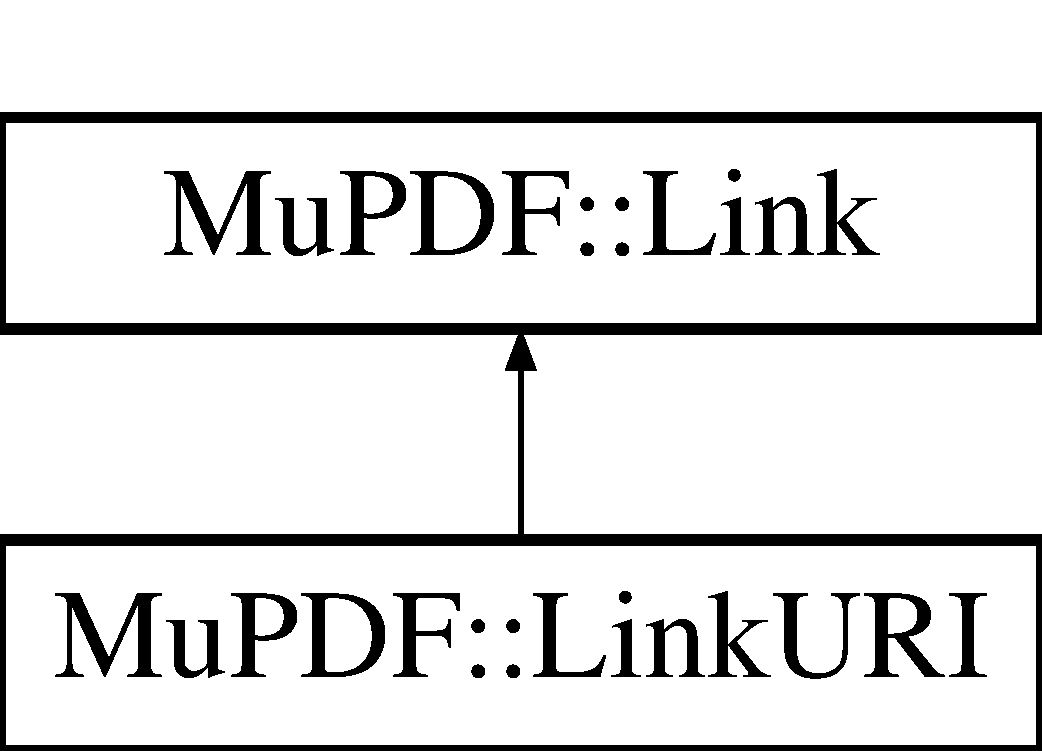
\includegraphics[height=2.000000cm]{class_mu_p_d_f_1_1_link_u_r_i}
\end{center}
\end{figure}
\subsection*{Public Member Functions}
\begin{DoxyCompactItemize}
\item 
\hyperlink{class_mu_p_d_f_1_1_link_afdc6828b6e00f323b53d6ae36d0d06b6}{Link\-Type} \hyperlink{class_mu_p_d_f_1_1_link_u_r_i_a32a9aea97620ed712100859e877597fe}{link\-Type} () const 
\item 
Q\-String \hyperlink{class_mu_p_d_f_1_1_link_u_r_i_a93ddf86fecab6a02abbcac0ef9a334d1}{uri} () const 
\begin{DoxyCompactList}\small\item\em A U\-T\-F-\/8 encoded U\-R\-I to launch. \end{DoxyCompactList}\item 
bool \hyperlink{class_mu_p_d_f_1_1_link_u_r_i_a6b567bf241449131f7ac5aafbcdd14cc}{is\-Map} () const 
\end{DoxyCompactItemize}
\subsection*{Friends}
\begin{DoxyCompactItemize}
\item 
class \hyperlink{class_mu_p_d_f_1_1_link_u_r_i_ab008ed670017e41b6e6bba8707c775d2}{Outline\-Item\-Private}
\end{DoxyCompactItemize}
\subsection*{Additional Inherited Members}


\subsection{Detailed Description}
A U\-R\-I link. 

Definition at line 59 of file mupdf-\/link.\-h.



\subsection{Member Function Documentation}
\hypertarget{class_mu_p_d_f_1_1_link_u_r_i_a6b567bf241449131f7ac5aafbcdd14cc}{\index{Mu\-P\-D\-F\-::\-Link\-U\-R\-I@{Mu\-P\-D\-F\-::\-Link\-U\-R\-I}!is\-Map@{is\-Map}}
\index{is\-Map@{is\-Map}!MuPDF::LinkURI@{Mu\-P\-D\-F\-::\-Link\-U\-R\-I}}
\subsubsection[{is\-Map}]{\setlength{\rightskip}{0pt plus 5cm}bool Mu\-P\-D\-F\-::\-Link\-U\-R\-I\-::is\-Map (
\begin{DoxyParamCaption}
{}
\end{DoxyParamCaption}
) const}}\label{class_mu_p_d_f_1_1_link_u_r_i_a6b567bf241449131f7ac5aafbcdd14cc}
If true, the x and y coords (as ints, in user space) should be appended to the U\-R\-I before launch. 

Definition at line 76 of file mupdf-\/link.\-cpp.

\hypertarget{class_mu_p_d_f_1_1_link_u_r_i_a32a9aea97620ed712100859e877597fe}{\index{Mu\-P\-D\-F\-::\-Link\-U\-R\-I@{Mu\-P\-D\-F\-::\-Link\-U\-R\-I}!link\-Type@{link\-Type}}
\index{link\-Type@{link\-Type}!MuPDF::LinkURI@{Mu\-P\-D\-F\-::\-Link\-U\-R\-I}}
\subsubsection[{link\-Type}]{\setlength{\rightskip}{0pt plus 5cm}{\bf Link\-Type} Mu\-P\-D\-F\-::\-Link\-U\-R\-I\-::link\-Type (
\begin{DoxyParamCaption}
{}
\end{DoxyParamCaption}
) const\hspace{0.3cm}{\ttfamily [inline]}, {\ttfamily [virtual]}}}\label{class_mu_p_d_f_1_1_link_u_r_i_a32a9aea97620ed712100859e877597fe}


Reimplemented from \hyperlink{class_mu_p_d_f_1_1_link_afe7888c7db760b5a77040cd075911c15}{Mu\-P\-D\-F\-::\-Link}.



Definition at line 62 of file mupdf-\/link.\-h.

\hypertarget{class_mu_p_d_f_1_1_link_u_r_i_a93ddf86fecab6a02abbcac0ef9a334d1}{\index{Mu\-P\-D\-F\-::\-Link\-U\-R\-I@{Mu\-P\-D\-F\-::\-Link\-U\-R\-I}!uri@{uri}}
\index{uri@{uri}!MuPDF::LinkURI@{Mu\-P\-D\-F\-::\-Link\-U\-R\-I}}
\subsubsection[{uri}]{\setlength{\rightskip}{0pt plus 5cm}Q\-String Mu\-P\-D\-F\-::\-Link\-U\-R\-I\-::uri (
\begin{DoxyParamCaption}
{}
\end{DoxyParamCaption}
) const}}\label{class_mu_p_d_f_1_1_link_u_r_i_a93ddf86fecab6a02abbcac0ef9a334d1}


A U\-T\-F-\/8 encoded U\-R\-I to launch. 



Definition at line 67 of file mupdf-\/link.\-cpp.



\subsection{Friends And Related Function Documentation}
\hypertarget{class_mu_p_d_f_1_1_link_u_r_i_ab008ed670017e41b6e6bba8707c775d2}{\index{Mu\-P\-D\-F\-::\-Link\-U\-R\-I@{Mu\-P\-D\-F\-::\-Link\-U\-R\-I}!Outline\-Item\-Private@{Outline\-Item\-Private}}
\index{Outline\-Item\-Private@{Outline\-Item\-Private}!MuPDF::LinkURI@{Mu\-P\-D\-F\-::\-Link\-U\-R\-I}}
\subsubsection[{Outline\-Item\-Private}]{\setlength{\rightskip}{0pt plus 5cm}friend class Outline\-Item\-Private\hspace{0.3cm}{\ttfamily [friend]}}}\label{class_mu_p_d_f_1_1_link_u_r_i_ab008ed670017e41b6e6bba8707c775d2}


Definition at line 69 of file mupdf-\/link.\-h.



The documentation for this class was generated from the following files\-:\begin{DoxyCompactItemize}
\item 
libmupdf-\/qt/\hyperlink{mupdf-link_8h}{mupdf-\/link.\-h}\item 
libmupdf-\/qt/\hyperlink{mupdf-link_8cpp}{mupdf-\/link.\-cpp}\end{DoxyCompactItemize}

\hypertarget{class_mu_p_d_f_1_1_outline}{\section{Mu\-P\-D\-F\-:\-:Outline Class Reference}
\label{class_mu_p_d_f_1_1_outline}\index{Mu\-P\-D\-F\-::\-Outline@{Mu\-P\-D\-F\-::\-Outline}}
}


A tree of the outline of a document (also known as table of contents).  




{\ttfamily \#include $<$mupdf-\/outline.\-h$>$}

\subsection*{Public Member Functions}
\begin{DoxyCompactItemize}
\item 
\hyperlink{class_mu_p_d_f_1_1_outline_a595999d446d98a2dcabf0b208fad0038}{$\sim$\-Outline} ()
\item 
\hyperlink{class_mu_p_d_f_1_1_outline_item}{Outline\-Item} \hyperlink{class_mu_p_d_f_1_1_outline_a5cb3d15517c68bed0486cd7a2a06c5db}{top\-Level\-Item} () const 
\begin{DoxyCompactList}\small\item\em Top level item. \end{DoxyCompactList}\end{DoxyCompactItemize}
\subsection*{Friends}
\begin{DoxyCompactItemize}
\item 
class \hyperlink{class_mu_p_d_f_1_1_outline_a883538034e58fc5c0de7d4e4cab3cef7}{Document}
\end{DoxyCompactItemize}


\subsection{Detailed Description}
A tree of the outline of a document (also known as table of contents). 

Definition at line 19 of file mupdf-\/outline.\-h.



\subsection{Constructor \& Destructor Documentation}
\hypertarget{class_mu_p_d_f_1_1_outline_a595999d446d98a2dcabf0b208fad0038}{\index{Mu\-P\-D\-F\-::\-Outline@{Mu\-P\-D\-F\-::\-Outline}!$\sim$\-Outline@{$\sim$\-Outline}}
\index{$\sim$\-Outline@{$\sim$\-Outline}!MuPDF::Outline@{Mu\-P\-D\-F\-::\-Outline}}
\subsubsection[{$\sim$\-Outline}]{\setlength{\rightskip}{0pt plus 5cm}Mu\-P\-D\-F\-::\-Outline\-::$\sim$\-Outline (
\begin{DoxyParamCaption}
{}
\end{DoxyParamCaption}
)}}\label{class_mu_p_d_f_1_1_outline_a595999d446d98a2dcabf0b208fad0038}


Definition at line 17 of file mupdf-\/outline.\-cpp.



\subsection{Member Function Documentation}
\hypertarget{class_mu_p_d_f_1_1_outline_a5cb3d15517c68bed0486cd7a2a06c5db}{\index{Mu\-P\-D\-F\-::\-Outline@{Mu\-P\-D\-F\-::\-Outline}!top\-Level\-Item@{top\-Level\-Item}}
\index{top\-Level\-Item@{top\-Level\-Item}!MuPDF::Outline@{Mu\-P\-D\-F\-::\-Outline}}
\subsubsection[{top\-Level\-Item}]{\setlength{\rightskip}{0pt plus 5cm}{\bf Outline\-Item} Mu\-P\-D\-F\-::\-Outline\-::top\-Level\-Item (
\begin{DoxyParamCaption}
{}
\end{DoxyParamCaption}
) const}}\label{class_mu_p_d_f_1_1_outline_a5cb3d15517c68bed0486cd7a2a06c5db}


Top level item. 



Definition at line 31 of file mupdf-\/outline.\-cpp.



\subsection{Friends And Related Function Documentation}
\hypertarget{class_mu_p_d_f_1_1_outline_a883538034e58fc5c0de7d4e4cab3cef7}{\index{Mu\-P\-D\-F\-::\-Outline@{Mu\-P\-D\-F\-::\-Outline}!Document@{Document}}
\index{Document@{Document}!MuPDF::Outline@{Mu\-P\-D\-F\-::\-Outline}}
\subsubsection[{Document}]{\setlength{\rightskip}{0pt plus 5cm}friend class {\bf Document}\hspace{0.3cm}{\ttfamily [friend]}}}\label{class_mu_p_d_f_1_1_outline_a883538034e58fc5c0de7d4e4cab3cef7}


Definition at line 31 of file mupdf-\/outline.\-h.



The documentation for this class was generated from the following files\-:\begin{DoxyCompactItemize}
\item 
/home/a/project/mupdf-\/qt/include/\hyperlink{mupdf-outline_8h}{mupdf-\/outline.\-h}\item 
/home/a/project/mupdf-\/qt/src/\hyperlink{mupdf-outline_8cpp}{mupdf-\/outline.\-cpp}\end{DoxyCompactItemize}

\hypertarget{class_mu_p_d_f_1_1_outline_item}{\section{Mu\-P\-D\-F\-:\-:Outline\-Item Class Reference}
\label{class_mu_p_d_f_1_1_outline_item}\index{Mu\-P\-D\-F\-::\-Outline\-Item@{Mu\-P\-D\-F\-::\-Outline\-Item}}
}


A outline item.  




{\ttfamily \#include $<$mupdf-\/outline.\-h$>$}

\subsection*{Public Member Functions}
\begin{DoxyCompactItemize}
\item 
\hyperlink{class_mu_p_d_f_1_1_outline_item_a7becb50f8c420c97e91ad7447db4352e}{Outline\-Item} ()
\item 
\hyperlink{class_mu_p_d_f_1_1_outline_item_a2b12873e1a87c12934f5f4b50db4b462}{Outline\-Item} (const \hyperlink{class_mu_p_d_f_1_1_outline_item}{Outline\-Item} \&item)
\item 
\hyperlink{class_mu_p_d_f_1_1_outline_item}{Outline\-Item} \& \hyperlink{class_mu_p_d_f_1_1_outline_item_acbb658a651ca336b1fc63ab638ebe2bb}{operator=} (const \hyperlink{class_mu_p_d_f_1_1_outline_item}{Outline\-Item} \&item)
\item 
\hyperlink{class_mu_p_d_f_1_1_outline_item_aaed50f784c03ff8b1e83cc14d15c6ebc}{$\sim$\-Outline\-Item} ()
\item 
bool \hyperlink{class_mu_p_d_f_1_1_outline_item_a0f8f4d3f59da951e5a9f4d467846d97f}{is\-Valid} () const 
\begin{DoxyCompactList}\small\item\em Whether this item is valid or not. \end{DoxyCompactList}\item 
Q\-String \hyperlink{class_mu_p_d_f_1_1_outline_item_a39279fb107effca0ee53f0931d06260d}{title} () const 
\begin{DoxyCompactList}\small\item\em Title. \end{DoxyCompactList}\item 
\hyperlink{class_mu_p_d_f_1_1_link}{Link} $\ast$ \hyperlink{class_mu_p_d_f_1_1_outline_item_afe6250e9dd784104369ed0f4178ed113}{link} () const 
\begin{DoxyCompactList}\small\item\em \hyperlink{class_mu_p_d_f_1_1_link}{Link}. \end{DoxyCompactList}\item 
\hyperlink{class_mu_p_d_f_1_1_outline_item}{Outline\-Item} \hyperlink{class_mu_p_d_f_1_1_outline_item_aac4d96f572743aab40916b45861ca914}{next} () const 
\begin{DoxyCompactList}\small\item\em The next outline item. \end{DoxyCompactList}\item 
\hyperlink{class_mu_p_d_f_1_1_outline_item}{Outline\-Item} \hyperlink{class_mu_p_d_f_1_1_outline_item_a3d74fe1a6ed39127f8326a8cfb4205f3}{down} () const 
\begin{DoxyCompactList}\small\item\em The down outline item. \end{DoxyCompactList}\end{DoxyCompactItemize}
\subsection*{Friends}
\begin{DoxyCompactItemize}
\item 
class \hyperlink{class_mu_p_d_f_1_1_outline_item_a3080a8e2042282b4224b6dc0a5d1cebe}{Outline}
\end{DoxyCompactItemize}


\subsection{Detailed Description}
A outline item. 

Definition at line 37 of file mupdf-\/outline.\-h.



\subsection{Constructor \& Destructor Documentation}
\hypertarget{class_mu_p_d_f_1_1_outline_item_a7becb50f8c420c97e91ad7447db4352e}{\index{Mu\-P\-D\-F\-::\-Outline\-Item@{Mu\-P\-D\-F\-::\-Outline\-Item}!Outline\-Item@{Outline\-Item}}
\index{Outline\-Item@{Outline\-Item}!MuPDF::OutlineItem@{Mu\-P\-D\-F\-::\-Outline\-Item}}
\subsubsection[{Outline\-Item}]{\setlength{\rightskip}{0pt plus 5cm}Mu\-P\-D\-F\-::\-Outline\-Item\-::\-Outline\-Item (
\begin{DoxyParamCaption}
{}
\end{DoxyParamCaption}
)}}\label{class_mu_p_d_f_1_1_outline_item_a7becb50f8c420c97e91ad7447db4352e}


Definition at line 37 of file mupdf-\/outline.\-cpp.

\hypertarget{class_mu_p_d_f_1_1_outline_item_a2b12873e1a87c12934f5f4b50db4b462}{\index{Mu\-P\-D\-F\-::\-Outline\-Item@{Mu\-P\-D\-F\-::\-Outline\-Item}!Outline\-Item@{Outline\-Item}}
\index{Outline\-Item@{Outline\-Item}!MuPDF::OutlineItem@{Mu\-P\-D\-F\-::\-Outline\-Item}}
\subsubsection[{Outline\-Item}]{\setlength{\rightskip}{0pt plus 5cm}Mu\-P\-D\-F\-::\-Outline\-Item\-::\-Outline\-Item (
\begin{DoxyParamCaption}
\item[{const {\bf Outline\-Item} \&}]{item}
\end{DoxyParamCaption}
)}}\label{class_mu_p_d_f_1_1_outline_item_a2b12873e1a87c12934f5f4b50db4b462}


Definition at line 54 of file mupdf-\/outline.\-cpp.

\hypertarget{class_mu_p_d_f_1_1_outline_item_aaed50f784c03ff8b1e83cc14d15c6ebc}{\index{Mu\-P\-D\-F\-::\-Outline\-Item@{Mu\-P\-D\-F\-::\-Outline\-Item}!$\sim$\-Outline\-Item@{$\sim$\-Outline\-Item}}
\index{$\sim$\-Outline\-Item@{$\sim$\-Outline\-Item}!MuPDF::OutlineItem@{Mu\-P\-D\-F\-::\-Outline\-Item}}
\subsubsection[{$\sim$\-Outline\-Item}]{\setlength{\rightskip}{0pt plus 5cm}Mu\-P\-D\-F\-::\-Outline\-Item\-::$\sim$\-Outline\-Item (
\begin{DoxyParamCaption}
{}
\end{DoxyParamCaption}
)}}\label{class_mu_p_d_f_1_1_outline_item_aaed50f784c03ff8b1e83cc14d15c6ebc}


Definition at line 74 of file mupdf-\/outline.\-cpp.



\subsection{Member Function Documentation}
\hypertarget{class_mu_p_d_f_1_1_outline_item_a3d74fe1a6ed39127f8326a8cfb4205f3}{\index{Mu\-P\-D\-F\-::\-Outline\-Item@{Mu\-P\-D\-F\-::\-Outline\-Item}!down@{down}}
\index{down@{down}!MuPDF::OutlineItem@{Mu\-P\-D\-F\-::\-Outline\-Item}}
\subsubsection[{down}]{\setlength{\rightskip}{0pt plus 5cm}{\bf Outline\-Item} Mu\-P\-D\-F\-::\-Outline\-Item\-::down (
\begin{DoxyParamCaption}
{}
\end{DoxyParamCaption}
) const}}\label{class_mu_p_d_f_1_1_outline_item_a3d74fe1a6ed39127f8326a8cfb4205f3}


The down outline item. 

\begin{DoxyReturn}{Returns}
a invalid outline item if there is no down outline item
\end{DoxyReturn}
\begin{DoxyNote}{Note}
The \hyperlink{class_mu_p_d_f_1_1_outline_item}{Outline\-Item} M\-U\-S\-T be valid. 
\end{DoxyNote}
\begin{DoxySeeAlso}{See Also}
\hyperlink{class_mu_p_d_f_1_1_outline_item_a0f8f4d3f59da951e5a9f4d467846d97f}{is\-Valid()} 
\end{DoxySeeAlso}


Definition at line 181 of file mupdf-\/outline.\-cpp.

\hypertarget{class_mu_p_d_f_1_1_outline_item_a0f8f4d3f59da951e5a9f4d467846d97f}{\index{Mu\-P\-D\-F\-::\-Outline\-Item@{Mu\-P\-D\-F\-::\-Outline\-Item}!is\-Valid@{is\-Valid}}
\index{is\-Valid@{is\-Valid}!MuPDF::OutlineItem@{Mu\-P\-D\-F\-::\-Outline\-Item}}
\subsubsection[{is\-Valid}]{\setlength{\rightskip}{0pt plus 5cm}bool Mu\-P\-D\-F\-::\-Outline\-Item\-::is\-Valid (
\begin{DoxyParamCaption}
{}
\end{DoxyParamCaption}
) const}}\label{class_mu_p_d_f_1_1_outline_item_a0f8f4d3f59da951e5a9f4d467846d97f}


Whether this item is valid or not. 



Definition at line 124 of file mupdf-\/outline.\-cpp.

\hypertarget{class_mu_p_d_f_1_1_outline_item_afe6250e9dd784104369ed0f4178ed113}{\index{Mu\-P\-D\-F\-::\-Outline\-Item@{Mu\-P\-D\-F\-::\-Outline\-Item}!link@{link}}
\index{link@{link}!MuPDF::OutlineItem@{Mu\-P\-D\-F\-::\-Outline\-Item}}
\subsubsection[{link}]{\setlength{\rightskip}{0pt plus 5cm}{\bf Link} $\ast$ Mu\-P\-D\-F\-::\-Outline\-Item\-::link (
\begin{DoxyParamCaption}
{}
\end{DoxyParamCaption}
) const}}\label{class_mu_p_d_f_1_1_outline_item_afe6250e9dd784104369ed0f4178ed113}


\hyperlink{class_mu_p_d_f_1_1_link}{Link}. 

\begin{DoxyNote}{Note}
Do not delete the returned pointer. It will be deleted automatically when \hyperlink{class_mu_p_d_f_1_1_outline_item}{Outline\-Item} is deleted. 

The \hyperlink{class_mu_p_d_f_1_1_outline_item}{Outline\-Item} M\-U\-S\-T be valid. 
\end{DoxyNote}
\begin{DoxySeeAlso}{See Also}
\hyperlink{class_mu_p_d_f_1_1_outline_item_a0f8f4d3f59da951e5a9f4d467846d97f}{is\-Valid()} 
\end{DoxySeeAlso}


Definition at line 148 of file mupdf-\/outline.\-cpp.

\hypertarget{class_mu_p_d_f_1_1_outline_item_aac4d96f572743aab40916b45861ca914}{\index{Mu\-P\-D\-F\-::\-Outline\-Item@{Mu\-P\-D\-F\-::\-Outline\-Item}!next@{next}}
\index{next@{next}!MuPDF::OutlineItem@{Mu\-P\-D\-F\-::\-Outline\-Item}}
\subsubsection[{next}]{\setlength{\rightskip}{0pt plus 5cm}{\bf Outline\-Item} Mu\-P\-D\-F\-::\-Outline\-Item\-::next (
\begin{DoxyParamCaption}
{}
\end{DoxyParamCaption}
) const}}\label{class_mu_p_d_f_1_1_outline_item_aac4d96f572743aab40916b45861ca914}


The next outline item. 

\begin{DoxyReturn}{Returns}
a invalid outline item if there is no next outline item
\end{DoxyReturn}
\begin{DoxyNote}{Note}
The \hyperlink{class_mu_p_d_f_1_1_outline_item}{Outline\-Item} M\-U\-S\-T be valid. 
\end{DoxyNote}
\begin{DoxySeeAlso}{See Also}
\hyperlink{class_mu_p_d_f_1_1_outline_item_a0f8f4d3f59da951e5a9f4d467846d97f}{is\-Valid()} 
\end{DoxySeeAlso}


Definition at line 161 of file mupdf-\/outline.\-cpp.

\hypertarget{class_mu_p_d_f_1_1_outline_item_acbb658a651ca336b1fc63ab638ebe2bb}{\index{Mu\-P\-D\-F\-::\-Outline\-Item@{Mu\-P\-D\-F\-::\-Outline\-Item}!operator=@{operator=}}
\index{operator=@{operator=}!MuPDF::OutlineItem@{Mu\-P\-D\-F\-::\-Outline\-Item}}
\subsubsection[{operator=}]{\setlength{\rightskip}{0pt plus 5cm}{\bf Outline\-Item} \& Mu\-P\-D\-F\-::\-Outline\-Item\-::operator= (
\begin{DoxyParamCaption}
\item[{const {\bf Outline\-Item} \&}]{item}
\end{DoxyParamCaption}
)}}\label{class_mu_p_d_f_1_1_outline_item_acbb658a651ca336b1fc63ab638ebe2bb}


Definition at line 63 of file mupdf-\/outline.\-cpp.

\hypertarget{class_mu_p_d_f_1_1_outline_item_a39279fb107effca0ee53f0931d06260d}{\index{Mu\-P\-D\-F\-::\-Outline\-Item@{Mu\-P\-D\-F\-::\-Outline\-Item}!title@{title}}
\index{title@{title}!MuPDF::OutlineItem@{Mu\-P\-D\-F\-::\-Outline\-Item}}
\subsubsection[{title}]{\setlength{\rightskip}{0pt plus 5cm}Q\-String Mu\-P\-D\-F\-::\-Outline\-Item\-::title (
\begin{DoxyParamCaption}
{}
\end{DoxyParamCaption}
) const}}\label{class_mu_p_d_f_1_1_outline_item_a39279fb107effca0ee53f0931d06260d}


Title. 

\begin{DoxyNote}{Note}
The \hyperlink{class_mu_p_d_f_1_1_outline_item}{Outline\-Item} M\-U\-S\-T be valid. 
\end{DoxyNote}
\begin{DoxySeeAlso}{See Also}
\hyperlink{class_mu_p_d_f_1_1_outline_item_a0f8f4d3f59da951e5a9f4d467846d97f}{is\-Valid()} 
\end{DoxySeeAlso}


Definition at line 135 of file mupdf-\/outline.\-cpp.



\subsection{Friends And Related Function Documentation}
\hypertarget{class_mu_p_d_f_1_1_outline_item_a3080a8e2042282b4224b6dc0a5d1cebe}{\index{Mu\-P\-D\-F\-::\-Outline\-Item@{Mu\-P\-D\-F\-::\-Outline\-Item}!Outline@{Outline}}
\index{Outline@{Outline}!MuPDF::OutlineItem@{Mu\-P\-D\-F\-::\-Outline\-Item}}
\subsubsection[{Outline}]{\setlength{\rightskip}{0pt plus 5cm}friend class {\bf Outline}\hspace{0.3cm}{\ttfamily [friend]}}}\label{class_mu_p_d_f_1_1_outline_item_a3080a8e2042282b4224b6dc0a5d1cebe}


Definition at line 56 of file mupdf-\/outline.\-h.



The documentation for this class was generated from the following files\-:\begin{DoxyCompactItemize}
\item 
/home/a/project/mupdf-\/qt/include/\hyperlink{mupdf-outline_8h}{mupdf-\/outline.\-h}\item 
/home/a/project/mupdf-\/qt/src/\hyperlink{mupdf-outline_8cpp}{mupdf-\/outline.\-cpp}\end{DoxyCompactItemize}

\hypertarget{class_mu_p_d_f_1_1_page}{\section{Mu\-P\-D\-F\-:\-:Page Class Reference}
\label{class_mu_p_d_f_1_1_page}\index{Mu\-P\-D\-F\-::\-Page@{Mu\-P\-D\-F\-::\-Page}}
}


{\ttfamily \#include $<$mupdf-\/page.\-h$>$}

\subsection*{Public Member Functions}
\begin{DoxyCompactItemize}
\item 
\hyperlink{class_mu_p_d_f_1_1_page_af319e925b5460b6b09a40aacd1d68347}{$\sim$\-Page} ()
\item 
bool \hyperlink{class_mu_p_d_f_1_1_page_a1f60d3a284731ac220a8717eb6a93167}{is\-Valid} () const 
\begin{DoxyCompactList}\small\item\em Check whether this page object is valid. \end{DoxyCompactList}\item 
Q\-Image \hyperlink{class_mu_p_d_f_1_1_page_a50c32d7917fe979dcf5404d378852556}{render\-Image} () const 
\begin{DoxyCompactList}\small\item\em Render page to Q\-Image. \end{DoxyCompactList}\item 
Q\-Rect \hyperlink{class_mu_p_d_f_1_1_page_afd724fcf89232f953315c76ec5a134b0}{size} () const 
\begin{DoxyCompactList}\small\item\em \hyperlink{class_mu_p_d_f_1_1_page}{Page} size at 72 dpi. \end{DoxyCompactList}\item 
void \hyperlink{class_mu_p_d_f_1_1_page_ac6768d64b88de1ccdd1fa0abb2724db0}{set\-Transparent\-Rendering} (bool enable)
\begin{DoxyCompactList}\small\item\em Whether to do transparent page rendering. This function modify setting of current page only. For global setting, use \hyperlink{class_mu_p_d_f_1_1_document_a8df89d0517437182406e2ba766402a3c}{Document\-::set\-Transparent\-Rendering()} instead. \end{DoxyCompactList}\item 
void \hyperlink{class_mu_p_d_f_1_1_page_a4f16778c9c61692834644d298b6ee77f}{set\-Background\-Color} (int r, int g, int b, int a=255)
\begin{DoxyCompactList}\small\item\em Set background color. This function modify setting of current page only. For global setting, use \hyperlink{class_mu_p_d_f_1_1_document_a0b9669def894d9164543e3367ae11d21}{Document\-::set\-Background\-Color()} instead. \end{DoxyCompactList}\item 
void \hyperlink{class_mu_p_d_f_1_1_page_a366b4f46b6f83a45afda029c81ca4d15}{set\-Transform} (float scale\-X, float scale\-Y, float rotation=0.\-0f)
\begin{DoxyCompactList}\small\item\em Set scale and rotation. \end{DoxyCompactList}\item 
Q\-String \hyperlink{class_mu_p_d_f_1_1_page_a40d3c45ab4ad02a07c9af726f14c97f3}{text} (float x0, float y0, float x1, float y1) const 
\begin{DoxyCompactList}\small\item\em Return the text in a rect. \end{DoxyCompactList}\item 
Q\-List$<$ \hyperlink{class_mu_p_d_f_1_1_text_box}{Text\-Box} $\ast$ $>$ \hyperlink{class_mu_p_d_f_1_1_page_a357731345081db20d209685a50cca27a}{text\-List} () const 
\begin{DoxyCompactList}\small\item\em Return all text boxes of the page. \end{DoxyCompactList}\end{DoxyCompactItemize}
\subsection*{Friends}
\begin{DoxyCompactItemize}
\item 
class \hyperlink{class_mu_p_d_f_1_1_page_a883538034e58fc5c0de7d4e4cab3cef7}{Document}
\end{DoxyCompactItemize}


\subsection{Detailed Description}


Definition at line 17 of file mupdf-\/page.\-h.



\subsection{Constructor \& Destructor Documentation}
\hypertarget{class_mu_p_d_f_1_1_page_af319e925b5460b6b09a40aacd1d68347}{\index{Mu\-P\-D\-F\-::\-Page@{Mu\-P\-D\-F\-::\-Page}!$\sim$\-Page@{$\sim$\-Page}}
\index{$\sim$\-Page@{$\sim$\-Page}!MuPDF::Page@{Mu\-P\-D\-F\-::\-Page}}
\subsubsection[{$\sim$\-Page}]{\setlength{\rightskip}{0pt plus 5cm}Mu\-P\-D\-F\-::\-Page\-::$\sim$\-Page (
\begin{DoxyParamCaption}
{}
\end{DoxyParamCaption}
)}}\label{class_mu_p_d_f_1_1_page_af319e925b5460b6b09a40aacd1d68347}


Definition at line 106 of file mupdf-\/page.\-cpp.



\subsection{Member Function Documentation}
\hypertarget{class_mu_p_d_f_1_1_page_a1f60d3a284731ac220a8717eb6a93167}{\index{Mu\-P\-D\-F\-::\-Page@{Mu\-P\-D\-F\-::\-Page}!is\-Valid@{is\-Valid}}
\index{is\-Valid@{is\-Valid}!MuPDF::Page@{Mu\-P\-D\-F\-::\-Page}}
\subsubsection[{is\-Valid}]{\setlength{\rightskip}{0pt plus 5cm}bool Mu\-P\-D\-F\-::\-Page\-::is\-Valid (
\begin{DoxyParamCaption}
{}
\end{DoxyParamCaption}
) const}}\label{class_mu_p_d_f_1_1_page_a1f60d3a284731ac220a8717eb6a93167}


Check whether this page object is valid. 



Definition at line 117 of file mupdf-\/page.\-cpp.

\hypertarget{class_mu_p_d_f_1_1_page_a50c32d7917fe979dcf5404d378852556}{\index{Mu\-P\-D\-F\-::\-Page@{Mu\-P\-D\-F\-::\-Page}!render\-Image@{render\-Image}}
\index{render\-Image@{render\-Image}!MuPDF::Page@{Mu\-P\-D\-F\-::\-Page}}
\subsubsection[{render\-Image}]{\setlength{\rightskip}{0pt plus 5cm}Q\-Image Mu\-P\-D\-F\-::\-Page\-::render\-Image (
\begin{DoxyParamCaption}
{}
\end{DoxyParamCaption}
) const}}\label{class_mu_p_d_f_1_1_page_a50c32d7917fe979dcf5404d378852556}


Render page to Q\-Image. 

\begin{DoxyReturn}{Returns}
This function will return a empty Q\-Image if failed. 
\end{DoxyReturn}


Definition at line 127 of file mupdf-\/page.\-cpp.

\hypertarget{class_mu_p_d_f_1_1_page_a4f16778c9c61692834644d298b6ee77f}{\index{Mu\-P\-D\-F\-::\-Page@{Mu\-P\-D\-F\-::\-Page}!set\-Background\-Color@{set\-Background\-Color}}
\index{set\-Background\-Color@{set\-Background\-Color}!MuPDF::Page@{Mu\-P\-D\-F\-::\-Page}}
\subsubsection[{set\-Background\-Color}]{\setlength{\rightskip}{0pt plus 5cm}void Mu\-P\-D\-F\-::\-Page\-::set\-Background\-Color (
\begin{DoxyParamCaption}
\item[{int}]{r, }
\item[{int}]{g, }
\item[{int}]{b, }
\item[{int}]{a = {\ttfamily 255}}
\end{DoxyParamCaption}
)}}\label{class_mu_p_d_f_1_1_page_a4f16778c9c61692834644d298b6ee77f}


Set background color. This function modify setting of current page only. For global setting, use \hyperlink{class_mu_p_d_f_1_1_document_a0b9669def894d9164543e3367ae11d21}{Document\-::set\-Background\-Color()} instead. 

\begin{DoxyNote}{Note}
This function will only work when page is not transparent. This function won't change content of your file, it only change the way you render the page.
\end{DoxyNote}

\begin{DoxyParams}{Parameters}
{\em r} & red channel \\
\hline
{\em g} & green channel \\
\hline
{\em b} & blue channel \\
\hline
{\em a} & alpha channel(default with non transparent) \\
\hline
\end{DoxyParams}


Definition at line 252 of file mupdf-\/page.\-cpp.

\hypertarget{class_mu_p_d_f_1_1_page_a366b4f46b6f83a45afda029c81ca4d15}{\index{Mu\-P\-D\-F\-::\-Page@{Mu\-P\-D\-F\-::\-Page}!set\-Transform@{set\-Transform}}
\index{set\-Transform@{set\-Transform}!MuPDF::Page@{Mu\-P\-D\-F\-::\-Page}}
\subsubsection[{set\-Transform}]{\setlength{\rightskip}{0pt plus 5cm}void Mu\-P\-D\-F\-::\-Page\-::set\-Transform (
\begin{DoxyParamCaption}
\item[{float}]{scale\-X, }
\item[{float}]{scale\-Y, }
\item[{float}]{rotation = {\ttfamily 0.0f}}
\end{DoxyParamCaption}
)}}\label{class_mu_p_d_f_1_1_page_a366b4f46b6f83a45afda029c81ca4d15}


Set scale and rotation. 


\begin{DoxyParams}{Parameters}
{\em scale\-X} & Scale for X direction. Default value\-: 1.\-0f; $>$1.\-0f\-: zoom in; $<$1.\-0f\-: zoom out. \\
\hline
{\em scale\-Y} & Scale for Y direction. Default value\-: 1.\-0f; $>$1.\-0f\-: zoom in; $<$1.\-0f\-: zoom out. \\
\hline
{\em rotation} & Degree of clockwise rotation. Range\-: \mbox{[}0.\-0f, 360.\-0f). \\
\hline
\end{DoxyParams}


Definition at line 269 of file mupdf-\/page.\-cpp.

\hypertarget{class_mu_p_d_f_1_1_page_ac6768d64b88de1ccdd1fa0abb2724db0}{\index{Mu\-P\-D\-F\-::\-Page@{Mu\-P\-D\-F\-::\-Page}!set\-Transparent\-Rendering@{set\-Transparent\-Rendering}}
\index{set\-Transparent\-Rendering@{set\-Transparent\-Rendering}!MuPDF::Page@{Mu\-P\-D\-F\-::\-Page}}
\subsubsection[{set\-Transparent\-Rendering}]{\setlength{\rightskip}{0pt plus 5cm}void Mu\-P\-D\-F\-::\-Page\-::set\-Transparent\-Rendering (
\begin{DoxyParamCaption}
\item[{bool}]{enable}
\end{DoxyParamCaption}
)}}\label{class_mu_p_d_f_1_1_page_ac6768d64b88de1ccdd1fa0abb2724db0}


Whether to do transparent page rendering. This function modify setting of current page only. For global setting, use \hyperlink{class_mu_p_d_f_1_1_document_a8df89d0517437182406e2ba766402a3c}{Document\-::set\-Transparent\-Rendering()} instead. 


\begin{DoxyParams}{Parameters}
{\em enable} & True\-: transparent; False\-: not transparent(default). \\
\hline
\end{DoxyParams}


Definition at line 233 of file mupdf-\/page.\-cpp.

\hypertarget{class_mu_p_d_f_1_1_page_afd724fcf89232f953315c76ec5a134b0}{\index{Mu\-P\-D\-F\-::\-Page@{Mu\-P\-D\-F\-::\-Page}!size@{size}}
\index{size@{size}!MuPDF::Page@{Mu\-P\-D\-F\-::\-Page}}
\subsubsection[{size}]{\setlength{\rightskip}{0pt plus 5cm}Q\-Rect Mu\-P\-D\-F\-::\-Page\-::size (
\begin{DoxyParamCaption}
{}
\end{DoxyParamCaption}
) const}}\label{class_mu_p_d_f_1_1_page_afd724fcf89232f953315c76ec5a134b0}


\hyperlink{class_mu_p_d_f_1_1_page}{Page} size at 72 dpi. 



Definition at line 214 of file mupdf-\/page.\-cpp.

\hypertarget{class_mu_p_d_f_1_1_page_a40d3c45ab4ad02a07c9af726f14c97f3}{\index{Mu\-P\-D\-F\-::\-Page@{Mu\-P\-D\-F\-::\-Page}!text@{text}}
\index{text@{text}!MuPDF::Page@{Mu\-P\-D\-F\-::\-Page}}
\subsubsection[{text}]{\setlength{\rightskip}{0pt plus 5cm}Q\-String Mu\-P\-D\-F\-::\-Page\-::text (
\begin{DoxyParamCaption}
\item[{float}]{x0, }
\item[{float}]{y0, }
\item[{float}]{x1, }
\item[{float}]{y1}
\end{DoxyParamCaption}
) const}}\label{class_mu_p_d_f_1_1_page_a40d3c45ab4ad02a07c9af726f14c97f3}


Return the text in a rect. 


\begin{DoxyParams}{Parameters}
{\em x0} & X coordinate of top left corner. \\
\hline
{\em y0} & Y coordinate of top left corner. \\
\hline
{\em x1} & X coordinate of bottom right corner. \\
\hline
{\em y1} & Y coordinate of bottom right corner. \\
\hline
\end{DoxyParams}


Definition at line 286 of file mupdf-\/page.\-cpp.

\hypertarget{class_mu_p_d_f_1_1_page_a357731345081db20d209685a50cca27a}{\index{Mu\-P\-D\-F\-::\-Page@{Mu\-P\-D\-F\-::\-Page}!text\-List@{text\-List}}
\index{text\-List@{text\-List}!MuPDF::Page@{Mu\-P\-D\-F\-::\-Page}}
\subsubsection[{text\-List}]{\setlength{\rightskip}{0pt plus 5cm}Q\-List$<$ {\bf Text\-Box} $\ast$ $>$ Mu\-P\-D\-F\-::\-Page\-::text\-List (
\begin{DoxyParamCaption}
{}
\end{DoxyParamCaption}
) const}}\label{class_mu_p_d_f_1_1_page_a357731345081db20d209685a50cca27a}


Return all text boxes of the page. 

\begin{DoxyNote}{Note}
The returned text boxes should be deleted when they are no longer used. 

Sizes of the returned text boxes are at 72 dpi, so they won't change when \hyperlink{class_mu_p_d_f_1_1_page_a366b4f46b6f83a45afda029c81ca4d15}{set\-Transform()} is called. 
\end{DoxyNote}


Definition at line 317 of file mupdf-\/page.\-cpp.



\subsection{Friends And Related Function Documentation}
\hypertarget{class_mu_p_d_f_1_1_page_a883538034e58fc5c0de7d4e4cab3cef7}{\index{Mu\-P\-D\-F\-::\-Page@{Mu\-P\-D\-F\-::\-Page}!Document@{Document}}
\index{Document@{Document}!MuPDF::Page@{Mu\-P\-D\-F\-::\-Page}}
\subsubsection[{Document}]{\setlength{\rightskip}{0pt plus 5cm}friend class {\bf Document}\hspace{0.3cm}{\ttfamily [friend]}}}\label{class_mu_p_d_f_1_1_page_a883538034e58fc5c0de7d4e4cab3cef7}


Definition at line 34 of file mupdf-\/page.\-h.



The documentation for this class was generated from the following files\-:\begin{DoxyCompactItemize}
\item 
include/\hyperlink{mupdf-page_8h}{mupdf-\/page.\-h}\item 
src/\hyperlink{mupdf-page_8cpp}{mupdf-\/page.\-cpp}\end{DoxyCompactItemize}

\chapter{File Documentation}
\hypertarget{mupdf-document_8cpp}{\section{libmupdf-\/qt/mupdf-\/document.cpp File Reference}
\label{mupdf-document_8cpp}\index{libmupdf-\/qt/mupdf-\/document.\-cpp@{libmupdf-\/qt/mupdf-\/document.\-cpp}}
}
{\ttfamily \#include \char`\"{}mupdf-\/document.\-h\char`\"{}}\\*
{\ttfamily \#include \char`\"{}mupdf-\/document\-\_\-p.\-h\char`\"{}}\\*
{\ttfamily \#include \char`\"{}mupdf-\/page.\-h\char`\"{}}\\*
{\ttfamily \#include \char`\"{}mupdf-\/page\-\_\-p.\-h\char`\"{}}\\*
{\ttfamily \#include \char`\"{}mupdf-\/outline.\-h\char`\"{}}\\*
{\ttfamily \#include \char`\"{}mupdf-\/outline\-\_\-p.\-h\char`\"{}}\\*
{\ttfamily \#include $<$mupdf/fitz.\-h$>$}\\*
{\ttfamily \#include $<$Q\-String$>$}\\*
{\ttfamily \#include $<$Q\-Date\-Time$>$}\\*
\subsection*{Namespaces}
\begin{DoxyCompactItemize}
\item 
\hyperlink{namespace_mu_p_d_f}{Mu\-P\-D\-F}
\end{DoxyCompactItemize}
\subsection*{Constant Groups}
\begin{DoxyCompactItemize}
\item 
\hyperlink{namespace_mu_p_d_f}{Mu\-P\-D\-F}
\end{DoxyCompactItemize}
\subsection*{Functions}
\begin{DoxyCompactItemize}
\item 
Document $\ast$ \hyperlink{namespace_mu_p_d_f_a5cf746094bc9648aca0d4a83e3ac44b3}{Mu\-P\-D\-F\-::load\-Document} (const Q\-String \&file\-Path)
\begin{DoxyCompactList}\small\item\em Load document. \end{DoxyCompactList}\item 
Document $\ast$ \hyperlink{namespace_mu_p_d_f_a294a09188a3dcab290679752dfc8d52b}{Mu\-P\-D\-F\-::load\-Document} (const Q\-Byte\-Array \&bytes)
\end{DoxyCompactItemize}

\hypertarget{mupdf-document_8h}{\section{/home/a/project/mupdf-\/qt/include/mupdf-\/document.h File Reference}
\label{mupdf-document_8h}\index{/home/a/project/mupdf-\/qt/include/mupdf-\/document.\-h@{/home/a/project/mupdf-\/qt/include/mupdf-\/document.\-h}}
}
{\ttfamily \#include $<$Q\-Byte\-Array$>$}\\*
\subsection*{Classes}
\begin{DoxyCompactItemize}
\item 
class \hyperlink{class_mu_p_d_f_1_1_document}{Mu\-P\-D\-F\-::\-Document}
\end{DoxyCompactItemize}
\subsection*{Namespaces}
\begin{DoxyCompactItemize}
\item 
\hyperlink{namespace_mu_p_d_f}{Mu\-P\-D\-F}
\end{DoxyCompactItemize}
\subsection*{Constant Groups}
\begin{DoxyCompactItemize}
\item 
\hyperlink{namespace_mu_p_d_f}{Mu\-P\-D\-F}
\end{DoxyCompactItemize}
\subsection*{Functions}
\begin{DoxyCompactItemize}
\item 
Document $\ast$ \hyperlink{namespace_mu_p_d_f_a5cf746094bc9648aca0d4a83e3ac44b3}{Mu\-P\-D\-F\-::load\-Document} (const Q\-String \&file\-Path)
\begin{DoxyCompactList}\small\item\em Load document. \end{DoxyCompactList}\item 
Document $\ast$ \hyperlink{namespace_mu_p_d_f_a294a09188a3dcab290679752dfc8d52b}{Mu\-P\-D\-F\-::load\-Document} (const Q\-Byte\-Array \&bytes)
\end{DoxyCompactItemize}

\hypertarget{mupdf-link_8cpp}{\section{src/mupdf-\/link.cpp File Reference}
\label{mupdf-link_8cpp}\index{src/mupdf-\/link.\-cpp@{src/mupdf-\/link.\-cpp}}
}
{\ttfamily \#include \char`\"{}mupdf-\/link.\-h\char`\"{}}\\*
{\ttfamily \#include \char`\"{}mupdf-\/link\-\_\-p.\-h\char`\"{}}\\*
{\ttfamily \#include $<$mupdf/fitz.\-h$>$}\\*
{\ttfamily \#include $<$Q\-Rect\-F$>$}\\*
{\ttfamily \#include $<$Q\-String$>$}\\*
\subsection*{Namespaces}
\begin{DoxyCompactItemize}
\item 
\hyperlink{namespace_mu_p_d_f}{Mu\-P\-D\-F}
\end{DoxyCompactItemize}
\subsection*{Constant Groups}
\begin{DoxyCompactItemize}
\item 
\hyperlink{namespace_mu_p_d_f}{Mu\-P\-D\-F}
\end{DoxyCompactItemize}

\hypertarget{mupdf-link_8h}{\section{include/mupdf-\/link.h File Reference}
\label{mupdf-link_8h}\index{include/mupdf-\/link.\-h@{include/mupdf-\/link.\-h}}
}
\subsection*{Classes}
\begin{DoxyCompactItemize}
\item 
class \hyperlink{class_mu_p_d_f_1_1_link}{Mu\-P\-D\-F\-::\-Link}
\item 
class \hyperlink{class_mu_p_d_f_1_1_link_goto}{Mu\-P\-D\-F\-::\-Link\-Goto}
\begin{DoxyCompactList}\small\item\em Goto a position in current file. \end{DoxyCompactList}\item 
class \hyperlink{class_mu_p_d_f_1_1_link_u_r_i}{Mu\-P\-D\-F\-::\-Link\-U\-R\-I}
\begin{DoxyCompactList}\small\item\em A U\-R\-I link. \end{DoxyCompactList}\item 
class \hyperlink{class_mu_p_d_f_1_1_link_launch}{Mu\-P\-D\-F\-::\-Link\-Launch}
\begin{DoxyCompactList}\small\item\em Launch a file (a document or a executable). \end{DoxyCompactList}\item 
class \hyperlink{class_mu_p_d_f_1_1_link_named}{Mu\-P\-D\-F\-::\-Link\-Named}
\begin{DoxyCompactList}\small\item\em Named action to perform. \end{DoxyCompactList}\item 
class \hyperlink{class_mu_p_d_f_1_1_link_goto_r}{Mu\-P\-D\-F\-::\-Link\-Goto\-R}
\begin{DoxyCompactList}\small\item\em Goto a position in another file. \end{DoxyCompactList}\end{DoxyCompactItemize}
\subsection*{Namespaces}
\begin{DoxyCompactItemize}
\item 
\hyperlink{namespace_mu_p_d_f}{Mu\-P\-D\-F}
\end{DoxyCompactItemize}
\subsection*{Constant Groups}
\begin{DoxyCompactItemize}
\item 
\hyperlink{namespace_mu_p_d_f}{Mu\-P\-D\-F}
\end{DoxyCompactItemize}

\hypertarget{mupdf-outline_8cpp}{\section{src/mupdf-\/outline.cpp File Reference}
\label{mupdf-outline_8cpp}\index{src/mupdf-\/outline.\-cpp@{src/mupdf-\/outline.\-cpp}}
}
{\ttfamily \#include \char`\"{}mupdf-\/outline.\-h\char`\"{}}\\*
{\ttfamily \#include \char`\"{}mupdf-\/outline\-\_\-p.\-h\char`\"{}}\\*
{\ttfamily \#include \char`\"{}mupdf-\/link.\-h\char`\"{}}\\*
{\ttfamily \#include \char`\"{}mupdf-\/link\-\_\-p.\-h\char`\"{}}\\*
{\ttfamily \#include \char`\"{}mupdf-\/document\-\_\-p.\-h\char`\"{}}\\*
{\ttfamily \#include $<$Q\-String$>$}\\*
\subsection*{Namespaces}
\begin{DoxyCompactItemize}
\item 
\hyperlink{namespace_mu_p_d_f}{Mu\-P\-D\-F}
\end{DoxyCompactItemize}
\subsection*{Constant Groups}
\begin{DoxyCompactItemize}
\item 
\hyperlink{namespace_mu_p_d_f}{Mu\-P\-D\-F}
\end{DoxyCompactItemize}

\hypertarget{mupdf-outline_8h}{\section{include/mupdf-\/outline.h File Reference}
\label{mupdf-outline_8h}\index{include/mupdf-\/outline.\-h@{include/mupdf-\/outline.\-h}}
}
\subsection*{Classes}
\begin{DoxyCompactItemize}
\item 
class \hyperlink{class_mu_p_d_f_1_1_outline}{Mu\-P\-D\-F\-::\-Outline}
\begin{DoxyCompactList}\small\item\em A tree of the outline of a document (also known as table of contents). \end{DoxyCompactList}\item 
class \hyperlink{class_mu_p_d_f_1_1_outline_item}{Mu\-P\-D\-F\-::\-Outline\-Item}
\begin{DoxyCompactList}\small\item\em A outline item. \end{DoxyCompactList}\end{DoxyCompactItemize}
\subsection*{Namespaces}
\begin{DoxyCompactItemize}
\item 
\hyperlink{namespace_mu_p_d_f}{Mu\-P\-D\-F}
\end{DoxyCompactItemize}
\subsection*{Constant Groups}
\begin{DoxyCompactItemize}
\item 
\hyperlink{namespace_mu_p_d_f}{Mu\-P\-D\-F}
\end{DoxyCompactItemize}

\hypertarget{mupdf-page_8cpp}{\section{src/mupdf-\/page.cpp File Reference}
\label{mupdf-page_8cpp}\index{src/mupdf-\/page.\-cpp@{src/mupdf-\/page.\-cpp}}
}
{\ttfamily \#include \char`\"{}mupdf-\/page.\-h\char`\"{}}\\*
{\ttfamily \#include \char`\"{}mupdf-\/page\-\_\-p.\-h\char`\"{}}\\*
{\ttfamily \#include \char`\"{}mupdf-\/document.\-h\char`\"{}}\\*
{\ttfamily \#include \char`\"{}mupdf-\/document\-\_\-p.\-h\char`\"{}}\\*
{\ttfamily \#include \char`\"{}mupdf-\/textbox.\-h\char`\"{}}\\*
{\ttfamily \#include \char`\"{}mupdf-\/textbox\-\_\-p.\-h\char`\"{}}\\*
{\ttfamily \#include $<$mupdf/fitz.\-h$>$}\\*
{\ttfamily \#include $<$Q\-Image$>$}\\*
{\ttfamily \#include $<$Q\-Size\-F$>$}\\*
\subsection*{Namespaces}
\begin{DoxyCompactItemize}
\item 
\hyperlink{namespace_mu_p_d_f}{Mu\-P\-D\-F}
\end{DoxyCompactItemize}
\subsection*{Constant Groups}
\begin{DoxyCompactItemize}
\item 
\hyperlink{namespace_mu_p_d_f}{Mu\-P\-D\-F}
\end{DoxyCompactItemize}
\subsection*{Functions}
\begin{DoxyCompactItemize}
\item 
Q\-Point\-F \hyperlink{namespace_mu_p_d_f_a40833e5e56d0d7d44cba455e4186d5e4}{Mu\-P\-D\-F\-::map\-To\-Origin} (const Q\-Point\-F \&pos, float scale\-X, float scale\-Y, float rotation=0.\-0f)
\begin{DoxyCompactList}\small\item\em Map from a transformed point to the original point. \end{DoxyCompactList}\item 
Q\-Size\-F \hyperlink{namespace_mu_p_d_f_ae91a73bb4e3e4c10eb54c07ab9be9cf7}{Mu\-P\-D\-F\-::map\-To\-Origin} (const Q\-Size\-F \&size, float scale\-X, float scale\-Y, float rotation=0.\-0f)
\begin{DoxyCompactList}\small\item\em Map from a transformed size to the original size. \end{DoxyCompactList}\item 
Q\-Rect\-F \hyperlink{namespace_mu_p_d_f_a2132cae17dab8f9896ec0c83f0c2173c}{Mu\-P\-D\-F\-::map\-To\-Origin} (const Q\-Rect\-F \&rect, float scale\-X, float scale\-Y, float rotation=0.\-0f)
\begin{DoxyCompactList}\small\item\em Map from a transformed rect to the original rect. \end{DoxyCompactList}\item 
Q\-Point\-F \hyperlink{namespace_mu_p_d_f_ad849bcc678dd57c1f12619f9554e6aba}{Mu\-P\-D\-F\-::map\-From\-Origin} (const Q\-Point\-F \&pos, float scale\-X, float scale\-Y, float rotation=0.\-0f)
\begin{DoxyCompactList}\small\item\em Map from a original point to the transformed point. \end{DoxyCompactList}\item 
Q\-Size\-F \hyperlink{namespace_mu_p_d_f_a6c6cac36e5a30ed75952a619b19d33aa}{Mu\-P\-D\-F\-::map\-From\-Origin} (const Q\-Size\-F \&size, float scale\-X, float scale\-Y, float rotation=0.\-0f)
\begin{DoxyCompactList}\small\item\em Map from a original size to the transformed size. \end{DoxyCompactList}\item 
Q\-Rect\-F \hyperlink{namespace_mu_p_d_f_a2f2a28dce44170175d3e9ba9601478ea}{Mu\-P\-D\-F\-::map\-From\-Origin} (const Q\-Rect\-F \&rect, float scale\-X, float scale\-Y, float rotation=0.\-0f)
\begin{DoxyCompactList}\small\item\em Map from a original rect to the transformed rect. \end{DoxyCompactList}\end{DoxyCompactItemize}

\hypertarget{mupdf-page_8h}{\section{/home/a/project/mupdf-\/qt/include/mupdf-\/page.h File Reference}
\label{mupdf-page_8h}\index{/home/a/project/mupdf-\/qt/include/mupdf-\/page.\-h@{/home/a/project/mupdf-\/qt/include/mupdf-\/page.\-h}}
}
{\ttfamily \#include $<$Q\-List$>$}\\*
\subsection*{Classes}
\begin{DoxyCompactItemize}
\item 
class \hyperlink{class_mu_p_d_f_1_1_page}{Mu\-P\-D\-F\-::\-Page}
\begin{DoxyCompactList}\small\item\em A page. \end{DoxyCompactList}\end{DoxyCompactItemize}
\subsection*{Namespaces}
\begin{DoxyCompactItemize}
\item 
\hyperlink{namespace_mu_p_d_f}{Mu\-P\-D\-F}
\end{DoxyCompactItemize}
\subsection*{Constant Groups}
\begin{DoxyCompactItemize}
\item 
\hyperlink{namespace_mu_p_d_f}{Mu\-P\-D\-F}
\end{DoxyCompactItemize}
\subsection*{Functions}
\begin{DoxyCompactItemize}
\item 
Q\-Point\-F \hyperlink{namespace_mu_p_d_f_a40833e5e56d0d7d44cba455e4186d5e4}{Mu\-P\-D\-F\-::map\-To\-Origin} (const Q\-Point\-F \&pos, float scale\-X, float scale\-Y, float rotation=0.\-0f)
\begin{DoxyCompactList}\small\item\em Map from a transformed point to the original point. \end{DoxyCompactList}\item 
Q\-Size\-F \hyperlink{namespace_mu_p_d_f_ae91a73bb4e3e4c10eb54c07ab9be9cf7}{Mu\-P\-D\-F\-::map\-To\-Origin} (const Q\-Size\-F \&size, float scale\-X, float scale\-Y, float rotation=0.\-0f)
\begin{DoxyCompactList}\small\item\em Map from a transformed size to the original size. \end{DoxyCompactList}\item 
Q\-Rect\-F \hyperlink{namespace_mu_p_d_f_a2132cae17dab8f9896ec0c83f0c2173c}{Mu\-P\-D\-F\-::map\-To\-Origin} (const Q\-Rect\-F \&rect, float scale\-X, float scale\-Y, float rotation=0.\-0f)
\begin{DoxyCompactList}\small\item\em Map from a transformed rect to the original rect. \end{DoxyCompactList}\item 
Q\-Point\-F \hyperlink{namespace_mu_p_d_f_ad849bcc678dd57c1f12619f9554e6aba}{Mu\-P\-D\-F\-::map\-From\-Origin} (const Q\-Point\-F \&pos, float scale\-X, float scale\-Y, float rotation=0.\-0f)
\begin{DoxyCompactList}\small\item\em Map from a original point to the transformed point. \end{DoxyCompactList}\item 
Q\-Size\-F \hyperlink{namespace_mu_p_d_f_a6c6cac36e5a30ed75952a619b19d33aa}{Mu\-P\-D\-F\-::map\-From\-Origin} (const Q\-Size\-F \&size, float scale\-X, float scale\-Y, float rotation=0.\-0f)
\begin{DoxyCompactList}\small\item\em Map from a original size to the transformed size. \end{DoxyCompactList}\item 
Q\-Rect\-F \hyperlink{namespace_mu_p_d_f_a2f2a28dce44170175d3e9ba9601478ea}{Mu\-P\-D\-F\-::map\-From\-Origin} (const Q\-Rect\-F \&rect, float scale\-X, float scale\-Y, float rotation=0.\-0f)
\begin{DoxyCompactList}\small\item\em Map from a original rect to the transformed rect. \end{DoxyCompactList}\end{DoxyCompactItemize}

\hypertarget{mupdf-qt_8h}{\section{libmupdf-\/qt/mupdf-\/qt.h File Reference}
\label{mupdf-qt_8h}\index{libmupdf-\/qt/mupdf-\/qt.\-h@{libmupdf-\/qt/mupdf-\/qt.\-h}}
}
{\ttfamily \#include \char`\"{}mupdf-\/document.\-h\char`\"{}}\\*
{\ttfamily \#include \char`\"{}mupdf-\/page.\-h\char`\"{}}\\*
{\ttfamily \#include \char`\"{}mupdf-\/link.\-h\char`\"{}}\\*
{\ttfamily \#include \char`\"{}mupdf-\/outline.\-h\char`\"{}}\\*

%--- End generated contents ---

% Index
\newpage
\phantomsection
\addcontentsline{toc}{part}{Index}
\printindex

\end{document}
